\RequirePackage{fix-cm}
%
%\documentclass{svjour3}                     % onecolumn (standard format)
%\documentclass[smallcondensed]{svjour3}     % onecolumn (ditto)
\documentclass[smallextended,natbib]{svjour3}       % onecolumn (second format)
  %\documentclass[twocolumn]{svjour3}          % twocolumn
  %
  \smartqed  % flush right qed marks, e.g. at end of proof

  % For the ORCID icon
  \usepackage{scalerel}
  \usepackage{tikz}
  \usetikzlibrary{svg.path}

  \definecolor{orcidlogocol}{HTML}{A6CE39}
  \tikzset{
    orcidlogo/.pic={
      \fill[orcidlogocol] svg{M256,128c0,70.7-57.3,128-128,128C57.3,256,0,198.7,0,128C0,57.3,57.3,0,128,0C198.7,0,256,57.3,256,128z};
      \fill[white] svg{M86.3,186.2H70.9V79.1h15.4v48.4V186.2z}
                   svg{M108.9,79.1h41.6c39.6,0,57,28.3,57,53.6c0,27.5-21.5,53.6-56.8,53.6h-41.8V79.1z M124.3,172.4h24.5c34.9,0,42.9-26.5,42.9-39.7c0-21.5-13.7-39.7-43.7-39.7h-23.7V172.4z}
                   svg{M88.7,56.8c0,5.5-4.5,10.1-10.1,10.1c-5.6,0-10.1-4.6-10.1-10.1c0-5.6,4.5-10.1,10.1-10.1C84.2,46.7,88.7,51.3,88.7,56.8z};
    }
  }

  \newcommand\orcidicon[1]{\href{https://orcid.org/#1}{\mbox{\scalerel*{
  
\begin{tikzpicture}[yscale=-1,transform shape]
  \pic{orcidlogo};
  \end{tikzpicture}
  }{|}}}}

  \usepackage{lineno, hyperref}
  \usepackage{array, pbox}
  \usepackage{mathtools}
  \usepackage{caption}
  \usepackage{subcaption}
  \usepackage{graphicx}

  % To use chinese characters
  \usepackage{CJKutf8}

  % To add an appendix page
  \usepackage[page, title]{appendix}

  % To insert commas into large numbers automatically
  \usepackage{siunitx}

  % To add research questions
  \usepackage{ntheorem}
  \theoremseparator{:}
  \newtheorem{rsq}{Research Question}

  % To add subrsq theorems
  \makeatletter
  \newcounter{subrsq} 
  \let\savedc@rsq\c@rsq
  \newenvironment{subrsq}
   {%
    \setcounter{subrsq}{0}%
    \stepcounter{rsq}%
    \edef\saved@rsq{\thersq}% Save the current value of rsq
    \let\c@rsq\c@subrsq     % Now rsq is subrsq
    \renewcommand{\thersq}{\saved@rsq\alph{rsq}}%
   }
   {}
  \newcommand{\normrsq}{%
    \let\c@rsq\savedc@rsq % revert to the old one
    \renewcommand\thersq{\arabic{rsq}}%
  } 
  \makeatother


  % To add the envelope symbol in Corresponding Author using % \Letter
  \usepackage{marvosym}

  % to add superscripts to mark the institute of authors
  % patch \maketitle:
  \newcommand*{\affaddr}[1]{#1} % No op here. Customize it for different styles.
  \newcommand*{\affmark}[1][*]{\textsuperscript{#1}}

  % For table formatting
  \usepackage{multirow}
  \usepackage[normalem]{ulem}
  \useunder{\uline}{\ul}{}

  % For landscape tables
  \usepackage{lscape}

  \modulolinenumbers[5]

  \journalname{Information Technology \& Tourism}

  \bibliographystyle{spbasic}

\begin{document}

\title{Cross-culture differences in tourists faced with Japanese hospitality: A text mining and natural language processing study of satisfaction and dissatisfaction factors in Chinese and Western cultures}

  \titlerunning{Cross-culture differences in tourists faced with Japanese hospitality: A text ...}

  \author{Elisa Claire Alem\'an Carre\'on \protect\affmark[1] \orcidicon{0000-0002-6437-0866} \and
          Hugo Alberto Mendoza Espa\~na                                   \protect\affmark[1] \and
          Hirofumi Nonaka                                                 \protect\affmark[1] \and
          Toru Hiraoka                                                    \protect\affmark[2]
  }

  \authorrunning{E. Alemán Carreón et al.}

  \institute{\Letter \hspace*{0.16em} Elisa Claire Alem\'an Carre\'on  \at
              % Nagaoka University of Technology, Nagaoka, Japan \\
              \hspace*{1em} \email{elisa.claire.aleman.carreon@gmail.com} \\
              \hspace*{1em} ORCID: 0000-0002-6437-0866 %\\
              % Corresponding Author %  \\
              % \emph{Present address:P.C. 940-2033, Ribbon Nagaoka B104, 1128-3 Kaminozoki-machi, Nagaoka, Niigata, Japan}
          \and
              \hspace*{1em} Hugo Alberto Mendoza Espa\~na \at
              % Nagaoka University of Technology, Nagaoka, Japan \\
              \hspace*{1em} \email{mendoza.espana@gmail.com}
          \and
              \hspace*{1em} Hirofumi Nonaka \at
              % Nagaoka University of Technology, Nagaoka, Japan \\
              \hspace*{1em} \email{nonaka@kjs.nagaokaut.ac.jp}
          \and
              \hspace*{1em} Toru Hiraoka \at
              % University of Nagasaki, Nagasaki, Japan \\
              \hspace*{1em} \email{hiraoka@sun.ac.jp}
          \and
              \at \affaddr{\affmark[1] \hspace*{0.15em} Nagaoka University of Technology, Nagaoka, Japan}
          \and
              \at \affaddr{\affmark[2] \hspace*{0.15em} University of Nagasaki, Nagasaki, Japan}
  }

  \date{Received: date / Accepted: date}
  % The correct dates will be entered by the editor

  \maketitle

\begin{abstract}

  % The Japanese spirit of hospitality and service, \textit{Omotenashi}, is known worldwide for its excellence. Recent years show a steady increase in international tourists coming to Japan. Chinese tourists, especially, have been steadily increasing. However, before the shift that has brought in a global perspective in recent years, most studies in tourist behavior were biased for the Western world. Previous research shows that different cultural backgrounds result in different expectations and, arguably, different satisfaction factors. Knowing this, a cross-cultural study of differences between Asian and Western cultures after the current boom in the Chinese economy in the environment of the high standard Japanese hospitality is fascinating. Will the top-grade hospitality of Japan influence both populations equally, or will their cultural differences set them apart? Will they be satisfied with the hotel's purely managerial attributes or be more concerned with environmental factors that hotel management cannot change? We bring light to these questions and the differences in each population's satisfaction and dissatisfaction factors. Taking advantage of Web 2.0, we applied Shannon's entropy to extract these factors automatically and then use them in an SVM to classify a more extensive data set. We found that Chinese tourists are less concerned with hospitality and more with room quality, in contrast with Western tourists, who were delighted by the staff behavior. We also found that Chinese tourists are concerned with the lack of a Chinese friendly environment, and Western customers are unsatisfied with dirty rooms or the smell of cigarettes.

  \keywords{Sentiment Analysis\and Hotels and Lodging\and Text Mining\and Chinese\and English\and Satisfaction and Dissatisfaction Factors}

\end{abstract}

\linenumbers

\section{Introduction}\label{intro}

  Japan has been known historically for its hospitality being the highest grade. The spirit of Japanese hospitality is celebrated around the world in a single Japanese word: \textit{Omotenashi}. With roots in Japanese history and tea ceremony, their hospitality is famous around the world \cite{al2015characteristics}. Therefore it would stand to reason that tourists visiting Japan would have this hospitality as their first and foremost satisfaction factor. However, it is known that customers from different countries and cultures hold different expectations \cite{engel1990}. Thus, it could be theorized that their satisfaction factors should be different. How will different cultures react and perceive hotels and their hospitality in this context? Our study attempts to bring light to this with two essential tourist populations that differ in culture to Japan: Chinese and Western tourists. 

  In the last couple of decades, the Japanese economy has been more and more affected by an increase in inbound international tourism \cite[][]{jones2009} with a Year-on-Year Growth Rate of 19.3\% in 2017, with a total of \num[group-separator={,}]{28691073} inbound tourists that year \cite[][]{jnto2003-2019}. From this total, the tourist population was mostly Asian (86.14\%), and approximately a fourth of the total (25.63\%) came from China. Western countries, counting English-speaking countries and the whole of Europe, make for 11.4\% of the total, with a 7.23\% of the total being countries where English is the official or the de facto national language. The effect of Chinese tourists on international economies is increasing. From that, the number of researchers interested in this phenomenon has been increasing as well. \cite[][]{sun2017}. With these and other multicultural tourist populations, the tourist market is more and more diverse. Diversity in customers' cultural backgrounds means that their expectations when staying at a hotel will also be varied. Hotel management, therefore, needs to cater to these needs and expectations to increase customer satisfaction, maintain a good reputation, and generate positive word-of-mouth.

  However, recent studies on social sciences, and thus, on tourist behavior, have been performed using surveys on populations that could be culturally biased for the western world \cite[][]{nielsen2017, jones2010WEIRD, guaratne2009, hogan1978biases}. Those that do include Asian populations in their analysis, most commonly study Chinese tourist behavior \cite[e.g.][]{liu2019, chang2010, dongyang2015}.  The few that compare Asian to western tourist behavior \cite[e.g.][]{choi2000} are commonly survey or interview-based studies with small samples, which, while valid, can have its limitations. This gap in research creates a need for cross-cultural studies for the increasing Asian and Western tourist populations. It could be said that Westerners make for a smaller portion of the tourist population compared to Asians. However, according to \cite{choi2000}, Westerners are known as ``long-haul" customers, spending more than 45\% of their budget on hotel lodging. In comparison, their Asian counterparts only spend 25\% of their budget on hotels. Therefore, it is essential to study both Asian and Western tourist populations, their differences, and contrast the results with existing literature. 

  With the advent of Web 2.0 and customer review websites, researchers realized the benefits of online reviews for research, and their importance for sales  \cite[][]{ye2009, basuroy2003}, customer consideration \cite[][]{vermeulen2009} and perception of services and products \cite[][]{browning2013}, among other effects of online interactions between customers \cite[e.g.][]{xiang2010, ren2019}. Consequentially, tourism research also began to use information collected online for data mining analysis, such as opinion mining \cite[e.g.][]{hu2017436}, predicting hotel demand from online traffic \cite[][]{yang2014}, recommender systems \cite[e.g.][]{loh2003}, and more. Data mining, machine learning, and big data methodologies can increase the number of manageable samples per study. The increase can be from the hundred samples manually analyzed by researchers to the hundreds of thousands that are automatically analyzed by machines. This technology can not only help confirm existing theories but also lead to finding new patterns and to knowledge discovery \cite[][]{fayyad1996data}. 

  In this study, we take advantage of the availability of enormous amounts of online reviews of Japanese hotels by both Mainland Chinese tourists posting in \textit{Ctrip} and Western English-speaking tourists populations posting in \textit{TripAdvisor}. With this data, we can confirm existing theories about their differences in behavior, as well as perform an exploration of the data to discover factors that could have been overlooked in the past. In order to do this, we use machine learning to automatically classify review sentences as positive or negative opinions of the hotel. We then perform a statistical extraction of the topics that concerns the customers of each population the most.

\section{Research objective}\label{research_objective}

  This study's objective is to determine the difference in factors driving satisfaction and dissatisfaction between Chinese and English-speaking tourists in the context of high-grade hospitality of Japanese hotels using text-mining techniques. We aim to contrast the satisfaction and dissatisfaction factors of both customer groups using natural language processing to study commonly used word pairings. More importantly, we also intend to measure how hard and soft attributes influence much satisfaction and dissatisfaction of both customer groups. We define hard attributes as those that are difficult to change by a hotel management without investing in infrastructure or real estate. In contrast, soft attributes are easily modifiable by improvements in management.

  Our proposal includes the use of large scale data from online hotel reviews in Chinese and English to study their differences in a statistical manner. In the past, survey-based studies have provided a theoretical background for a few specific tourist populations of a single culture or that travel with a single purpose. The short scope of those studies means that cultural and language differences often cannot be observed in a single study. 

  Our study attempts to uncover the difference in satisfaction and dissatisfaction factors between cultures. These factors can become the focal point for making improvements in the tourism and service industries and increase customer satisfaction. Satisfied customers will then write more positive online reviews that will, in turn, increase sales and attract new customers. 

\section{Theoretical background and hypothesis development}\label{theory_hypothesis}

  \subsection{Japanese hospitality: \textit{Omotenashi}}\label{theory_omotenashi}

    The spirit of Japanese hospitality, or \textit{Omotenashi}, has roots in the countries history. However, to this day, it is regarded as the highest standard \cite[][]{ikeda2013omotenashi, al2015characteristics}. There is even a famous phrase in customer service in Japan: \textit{okyaku-sama wa kami-sama desu}, or translated ``The customer is god''. Some say that \textit{Omotenashi} originated from the old Japanese art of the tea ceremony in the 16th century. However, other scholars found that its roots come from even earlier, in the form of formal banquets in the 7th century \cite[][]{aishima2015origin}. The practice of high standards in hospitality has survived throughout the years. Today, it permeates all business practices in Japan, from the cheapest convenience stores to the most expensive ones. Manners, service, and respect towards the customer are taught to workers in their training, and high standards are always followed as to not fall behind in the competition. In Japanese businesses, hotels included, staff members are trained to speak in \textit{sonkeigo}, or ``respectful language", one of the most formal of the Japanese formality syntaxes. They are also trained to bow with different depths depending on the situation, where a light bow could be used to say: ``Please, allow me to guide you". Deep bows are also used to apologize for any inconvenience the customer could have, followed by a very respectful apology as well. In fact, despite the word \textit{omotenashi} being translated directly as ``hospitality'', it includes both the concepts of hospitality and service \cite[][]{Kuboyama2020}. 

    It stands to reason that this high level of hospitality would be a positive aspect that would be at the top of satisfaction for any customer. However, in Japan, every business has this high level of hospitality, in differing levels of success. A simple convenience shop around the corner could be more hospitable if hotel management falls behind. Businesses have to strive to be the most hospitable, and hotels are not allowed to lag in this competition. Because of this, other factors such as proximity to a convenience store, or transport availability, or perhaps room quality might be more critical to a customer. Customers can always achieve satisfaction from hospitality elsewhere, so hotels need to be competitive in their hospitality. 

    Therefore we pose a research question for our study:

    \begin{subrsq}
    \begin{rsq}
    \label{rsq:omotenashi}
    To what degree are Chinese and Western tourists satisfied with Japanese \textit{Omotenashi} factors such as staff behavior or service?
    \end{rsq}

    However, Japanese hospitality comes from Japanese culture. Different cultures interacting with it could have a different reaction. While some might be impressed by it, some might consider other factors more important to their stay in a hotel. This point leads us to a derivative of the above research question:

    \begin{rsq}
    \label{rsq:omotenashi_both}
    Do Western and Chinese tourists have a different reaction to Japanese \textit{Omotenashi} factors such as staff behavior or service?
    \end{rsq}
    \end{subrsq}

  \subsection{Customer satisfaction and dissatisfaction during hotel lodging}\label{theory_satisfaction}

    Customer satisfaction in tourism has been analyzed since decades past, \cite{hunt1975} having defining customer satisfaction as the realization or overcoming of expectations towards the service. \cite{oliver1981} defined it as an emotional response to the provided services in retail and other contexts, and \cite{oh1996} reviewed the psychological processes of customer satisfaction for the hospitality industry. It is generally agreed upon that satisfaction and dissatisfaction stem from the individual expectations of the customer. As such, \cite{engel1990} states that each customer's background, therefore, influences satisfaction and dissatisfaction. Western and Chinese customers can then have very different factors of satisfaction and dissatisfaction since they have different backgrounds and cultures. These varying backgrounds will lead to varying expectations of the hotel services, the experiences they want to have while staying at a hotel, and the level of comfort that they will have. These expectations will be there from the moment that they choose the hotel throughout their stay. These different expectations, in turn, will determine the distinct factors of satisfaction and dissatisfaction for each kind of customer, as well as the order in which they prioritize them. 

    Because of their different origins, expectations, and cultures, it stands to reason Chinese and Western tourists could have completely different factors to one another. Therefore, it could be that some factors do not appear in the other reviews at all. For example, between different cultures, it can be that a single word can express some concept that would take more words in the other language. So we must measure their differences or similarities at their common ground as well. 

    Studies on customer satisfaction \cite[e.g.][]{truong2009, romao2014, wu2009} commonly use the Likert scale \cite[][]{likert1932technique} (e.g. 1 to 5 scale from strongly dissatisfied to strongly satisfied) to perform statistical analysis of which factors relate most to satisfaction on the same dimension as dissatisfaction \cite[e.g.][]{chan201518, choi2000}. The use of the Likert scale leads to correlation analyses where one factor can lead to satisfaction, implying that the lack of it can lead to dissatisfaction. However, a binary distinction (satisfied or dissatisfied) could allow us to analyze the factors that correlate to satisfaction and explore factors that are solely linked to dissatisfaction. There are fewer examples of this approach, but studies have done this in the past \cite[e.g.][]{zhou2014}. This method can indeed decrease the extent to which we can analyze degrees of satisfaction or dissatisfaction. However, it has the benefit that it can be applied to a large sample of text data via automatic sentiment detection techniques using artificial intelligence. 

    Previous research has also focused on soft attributes that are controllable by the hotel managers and staff, i.e., hotel services, staff behavior, or facilities \cite[e.g.][]{shanka2004, choi2001}. However, little focus is put on hard factors that are uncontrollable by the hotel staff that can play a part in the customers' choice behavior and satisfaction. Examples of these factors include the surroundings of the hotel, location, language immersion of the country as a whole, or touristic destinations, as well as the integration of the hotel with tours available nearby, among other factors. 

    This leads to another research question:

    \begin{rsq}
    \label{rsq:hard_soft}
    To what degree does satisfaction and dissatisfaction stem from hard and soft attributes of the hotel.
    \end{rsq}

    The resulting proportions of hard attributes to soft attributes for each population could serve as a measurement of how much the improvement of management in the hotel can increase future satisfaction in customers.

  \subsection{Chinese and Western tourist behavior}\label{theory_zh_en}

    % Asians vs. Western behavior
    In the past, tourist behavior analyzed from western samples was wrongly thought to be a representation of universal behavior across all cultures \cite[][]{nielsen2017, jones2010WEIRD, guaratne2009, hogan1978biases}. Recently, however, with the rise of Chinese outbound tourism, both academic researchers and businesses have decided to study Chinese tourist behavior \cite[][]{sun2017}. This increase resulted in several studies focusing on only the behavior of this subset of tourists. To this day, cross-cultural studies and analyses for Asian and Western tourists are scarce. One example is \cite{choi2000}, where it was found that Western tourists visiting Hong Kong are satisfied more with room quality while Asians are satisfied with value for money. Another is  \cite{bauer1993changing}, where Westerners prefer the hotel health facilities while the Asian tourists were more inclined to enjoy the Karaoke facilities of hotels, and both groups tend to have high expectations about the overall facilities. Another example is \cite{kim2000}, where American tourists were found to be individualistic and motivated by novelty, while Japanese tourists were found to be collectivist and motivated by prestige and family, with an escape from routine and an increase in knowledge as a common motivator. 

    One thing to note with the above cross-culture analyses is that they were performed before the year 2000. The current Chinese economy boom is making an increase in the influx of tourists. However, that boom could have created a difference in the expectations of tourists. In turn, that boom could have influenced their satisfaction factors when traveling. Another note is that these studies were performed with questionnaires in places where it would be easy to locate tourists, i.e., airports. However, our study of online reviews takes the data that the hotel customers uploaded themselves.

    More recent studies have surfaced as well. A cross-country study \cite{FRANCESCO201924} using posts from U.S.A. citizens, Italians and Chinese tourists, determined using a text link analysis that customers from different countries indeed have a different perception and emphasis of a few predefined hotel attributes. According to their results, it appears that U.S.A. customers perceive cleanliness and quietness most positively and that Chinese customers perceive budget and restaurant above other attributes. Another couple of studies \cite{JIA2020104071, HUANG2017117} analyze differences between Chinese and U.S. tourists using text mining techniques and more massive datasets, although in a restaurant context. 

    These last three articles focus on U.S.A. culture, while our study focuses on Western culture. Another difference with our study is that of the context of the study. The first study \cite{FRANCESCO201924} has the context of tourists from three countries staying in hotels across the world, the second choosing restaurant reviews from the U.S.A. and Chinese tourists eating in three countries in Europe, and the third analyzing reviews of restaurants in Bejing. Our study, on the other hand, focuses on Western culture, instead of a single Western country, and Chinese culture clashing with the hospitality environment in Japan, specifically. The importance of Japan in this analysis comes from the unique environment of high-grade hospitality that the country presents. In this environment, do customers hold their satisfaction to this hospitality regardless of their culture, or are other factors are more important to the customers overall? Our study measures this at a large scale across different hotels in Japan. 

    % Universal behavior
    Other studies, perhaps recognizing that samples being comprised of people from Western industrialized countries are not representative, have gone further and studied people from many countries in their samples, and performed a more universal and holistic (not cross-culture) analysis. \cite{choi2001}, for example, analyzed hotel guest satisfaction determinants in Hong Kong with surveys in English, Chinese and Japanese translations, with people from many countries in their sample. \cite{choi2001} found that staff service quality, room quality, and value for money were the top satisfaction determinants. As another example, \cite{Uzama2012} produced a typology for foreigners coming to Japan for tourism, without making distinctions for their culture, but their motivation in traveling in Japan. In another study, \cite{zhou2014} analyzed hotel satisfaction using English and Mandarin online reviews from guests staying in Hangzhou, China coming from many different countries. The general satisfaction score was noticed to be different in those countries. However, a more in-depth cross-cultural analysis of the satisfaction factors wasn't performed. As a result of their research, \cite{zhou2014} thus found that customers are universally satisfied by welcome extras, dining environments, and special food services. 

    % Western behavior 
    Regarding Western tourist behavior, a few examples can tell us what to expect when analyzing our data. \cite{kozak2002} found that British and German tourists' satisfaction determinants while visiting Spain and Turkey were hygiene and cleanliness, hospitality, the availability of facilities and activities, and accommodation services. \cite{shanka2004} found that English-speaking tourists in Perth, Australia were most satisfied with staff friendliness, the efficiency of check-in and check-out, restaurant and bar facilities, and lobby ambiance. 

    % Chinese behavior
    Regarding outbound Chinese tourists, academic studies about Chinese tourists have increased \cite[][]{sun2017}. Different researchers have found that Chinese tourist populations have several specific attributes. According to \cite{ryan2001} and their study of Chinese tourists in New Zealand, Chinese tourists prefer nature, cleanliness, and scenery in contrast to experiences and activities. \cite{dongyang2015} studied Chinese tourists in the Kansai region of Japan and found that Chinese tourists are satisfied mostly with exploring the food culture of their destination, cleanliness, and staff. Studying Chinese tourists in Vietnam, \cite{truong2009} found that Chinese tourists are highly concerned with value for money. According to \cite{liu2019}, Chinese tourists tend to have harsher criticism when compared with other international tourists. Moreover, as stated by \cite{gao2017chinese}, who analyzed different generations of Chinese tourists and their connection to nature while traveling, Chinese tourists prefer nature overall. However, the younger generations seem to do so less than their older counterparts. 

    % Studies are not universal.
    Although the studies focusing only on Chinese tourists or only on Western tourists have a narrow view, their theoretical contributions are valuable. We can see that depending on the study and the design of questionnaires, as well as the destinations; the results can vary greatly. Not only that, but while there seems to be some overlap in most studies, some factors are completely ignored in one study but not in the other. Since our study uses data mining, the definition of each factor is left for hotel customers to decide en masse via their reviews. This means that the factors will be selected through statistical methods alone, instead of being defined by the questionnaire. Our method allows us to find factors that we would not have contemplated. It also avoids enforcing a factor on the mind of study subjects by presenting them with a question that they did not think of by themselves. This large variety of opinions in a well-sized sample, added to the automatic findings of statistical text analysis methods, gives an advantage to our study compared to others with smaller samples. Besides, this study could help us analyze the satisfaction and dissatisfaction factors cross-culturally and compare them with the existing literature.

    % Reviewer comparison table
    Undoubtedly previous literature has examples of other cross-culture studies of tourist behavior and to further highlight our study and its merits. A contrast is shown in Table \ref{tab:lit-rev}. This table shows that older studies were conducted with surveys and had a different study topic. These are changes in demand \cite{bauer1993changing}, tourist motivation \cite{kim2000}, and closer to our study, satisfaction levels \cite{choi2000}. However, our study topic is not the levels of satisfaction but the factors that drive it, as well as dissatisfaction, which is overlooked in most studies. Newer studies with larger samples and similar methodologies have emerged, although two of these study restaurants instead of hotels \cite{JIA2020104071, HUANG2017117}. One important difference is the geographical focus of their studies. While \cite{FRANCESCO201924, JIA2020104071, HUANG2017117} have a multi-national focus, we instead focus on Japan. The focus on Japan is important because of its leading rank in hospitality across all types of businesses. This raises the question: in such an environment, will the customers be universally satisfied with this factor, or will they have differing views within their cultures? Our study brings light to the changes, or lack thereof, in different touristic environments where an attribute can be considered as excellent. The number of samples in other text-mining studies is also smaller to ours in comparison. Apart from that, every study has a different text mining method.

    % Please add the following required packages to your document preamble:
    % \usepackage{graphicx}
    % \usepackage{lscape}
    \begin{landscape}
    \begin{table}[htp]
    \centering
    \caption{Comparison between cross-culture or cross-country previous studies and our study.}
    \label{tab:lit-rev}
    \resizebox{\linewidth}{!}{%
    \begin{tabular}{l|l|l|l|l|l|l|l|}
    \cline{2-8}
    \textbf{} &
      \textbf{Bauer et.al (1993)} &
      \textbf{Choi and Chu (2000)} &
      \textbf{Kim and Lee (2000)} &
      \textbf{Huang (2017)} &
      \textbf{Francesco and Roberta (2019)} &
      \textbf{Jia (2020)} &
      \textbf{Our study} \\ \hline
    \multicolumn{1}{|l|}{\textbf{Comparison objects}} &
      \begin{tabular}[c]{@{}l@{}}Asians\\ vs\\ Westerns\end{tabular} &
      \begin{tabular}[c]{@{}l@{}}Asians\\ vs\\ Westerners\end{tabular} &
      \begin{tabular}[c]{@{}l@{}}Anglo-Americans \\ vs \\ Japanese\end{tabular} &
      \begin{tabular}[c]{@{}l@{}}Chinese \\ vs \\ English-speakers\end{tabular} &
      \begin{tabular}[c]{@{}l@{}}USA \\ vs \\ China \\ vs \\ Italy\end{tabular} &
      \begin{tabular}[c]{@{}l@{}}Chinese \\ vs \\ US tourists\end{tabular} &
      \begin{tabular}[c]{@{}l@{}}Chinese \\ vs \\ Westerners\end{tabular} \\ \hline
    \multicolumn{1}{|l|}{\textbf{Study topic}} &
      Changes in demand &
      Satisfaction Levels &
      Tourist Motivation &
      \begin{tabular}[c]{@{}l@{}}Dining experience \\ of Roast Duck\end{tabular} &
      \begin{tabular}[c]{@{}l@{}}Perception and \\ Emphasis\end{tabular} &
      \begin{tabular}[c]{@{}l@{}}Motivation and \\ Satisfaction\end{tabular} &
      \textbf{\begin{tabular}[c]{@{}l@{}}Satisfaction and\\ Dissatisfaction\end{tabular}} \\ \hline
    \multicolumn{1}{|l|}{\textbf{Geographical focus}} &
      Asia Pacific region &
      Hong Kong &
      Global &
      Beijing &
      Multi-national &
      Multi-national &
      \textbf{Japan} \\ \hline
    \multicolumn{1}{|l|}{\textbf{Industry}} &
      Hotels &
      Hotels &
      Tourism &
      Restaurant (Beijing Roast Duck) &
      Hotels &
      Restaurants &
      Hotels \\ \hline
    \multicolumn{1}{|l|}{\textbf{Study subjects}} &
      Hotel managers &
      Hotel customers &
      \begin{tabular}[c]{@{}l@{}}Tourists arriving \\ in airport\end{tabular} &
      \begin{tabular}[c]{@{}l@{}}Diners \\ online reviews\end{tabular} &
      \begin{tabular}[c]{@{}l@{}}Hotel customers \\ online reviews\end{tabular} &
      \begin{tabular}[c]{@{}l@{}}Diners \\ online reviews\end{tabular} &
      \begin{tabular}[c]{@{}l@{}}Hotel customers \\ online reviews\end{tabular} \\ \hline
    \multicolumn{1}{|l|}{\textbf{Sample method}} &
      surveys &
      surveys &
      survey &
      text mining &
      text mining &
      text mining &
      text mining \\ \hline
    \multicolumn{1}{|l|}{\textbf{Number of samples}} &
      185 surveys &
      540 surveys &
      \begin{tabular}[c]{@{}l@{}}165 Anglo-American\\ 209 Japanese\end{tabular} &
      \begin{tabular}[c]{@{}l@{}}990 Chinese reviews\\ 398 English reviews\end{tabular} &
      9000 reviews (3000 per country) &
      \begin{tabular}[c]{@{}l@{}}2448 reviews\\ (1360 Chinese)\\ (1088 English)\end{tabular} &
      \textbf{\begin{tabular}[c]{@{}l@{}}89,207 reviews\\ (48,070 Chinese)\\ (41,137 English)\end{tabular}} \\ \hline
    \multicolumn{1}{|l|}{\textbf{Study method}} &
      statistics &
      VARIMAX &
      MANOVA &
      \begin{tabular}[c]{@{}l@{}}Semantic \\ Network \\ Analysis\end{tabular} &
      Text Link Analysis &
      \begin{tabular}[c]{@{}l@{}}Topic modeling \\ (LDA)\end{tabular} &
      \textbf{\begin{tabular}[c]{@{}l@{}}SVM, \\ Dependency Parsing\\ and POS tagging\end{tabular}} \\ \hline
    \multicolumn{1}{|l|}{\textbf{Subject nationality}} &
      \begin{tabular}[c]{@{}l@{}}Asians: \\ China,\\ Fiji,\\ Hong Kong,\\ Indonesia,\\ Malaysia,\\ Singapore,\\ Taiwan,\\ Guam,\\ Tahiti,\\ Thailand \\ \\ Westerners: Australia,\\ New Zealand\end{tabular} &
      \begin{tabular}[c]{@{}l@{}}Asians:\\ China,\\ Taiwan,\\ Japan,\\ South Korea,\\ South-East Asia\\ \\ Westerners:\\ North America,\\ Europe,\\ Australia,\\ New Zealand\end{tabular} &
      USA, Japan &
      \begin{tabular}[c]{@{}l@{}}English-speakers: \\ U.K., U.S., Australia,\\ New Zealand, Canada,\\ Ireland\\ \\ Chinese-speakers: China\end{tabular} &
      USA, China, Italy &
      USA, China &
      \begin{tabular}[c]{@{}l@{}}Chinese-speakers:\\ China\\ \\ English-speakers:\\ (U.K., U.S.,\\ Australia,\\ New Zealand,\\ Canada, Ireland)\end{tabular} \\ \hline
    \end{tabular}%
    }
    \end{table}
    \end{landscape}

  \subsection{Data mining, machine learning, knowledge discovery and sentiment analysis}\label{theory_data}

    % Explain the discovery of theory inside the data
    In the current world, data is presented to us in larger and larger quantities. Today's data sizes were commonly only seen in very specialized large laboratories with supercomputers a couple of decades ago. However, they are now standard for market and managerial studies, independent university students, and any scientist that can connect to the Internet. Such quantities of data are available to study now more than ever. Nevertheless, it would be impossible for researchers to parse all of this data by themselves. As \cite{fayyad1996data} summarizes, data by itself is unusable until it goes through a process of selection, preprocessing, transformation, mining, and evaluation. Only then can it be established as knowledge. With the tools available to us in the era of information science, algorithms can be used to detect patterns that would take researchers too long to recognize. These patterns can, later on, be evaluated to generate knowledge. This process is called Knowledge Discovery in Databases. 

    % Text mining 
    Now, there are, of course, many sources of numerical data to be explored.  However, perhaps what is most available and interesting to managerial purposes is the resource of customers' opinions in text form. Since the introduction of Web 2.0, a never before seen quantity of valuable information is posted to the Internet at a staggering speed. Text mining has then been proposed more than a decade ago to utilize this data \cite[e.g.][]{rajman1998text,nahm2002text}. Using Natural Language Processing, one can parse language in a way that translates to numbers so that a computer can analyze it. Since then, text mining techniques have improved over the years. This has been used in the field of hospitality as well for many purposes, including satisfaction analysis from reviews \cite[e.g][]{berezina2016, xu2016, xiang2015, hargreaves2015, balbi2018}, social media's influence on travelers \cite[e.g.][]{xiang2010}, review summarization \cite[e.g.][]{hu2017436}, perceived value of reviews \cite[e.g][]{FANG2016498}, and even predicting hotel demand using web traffic data \cite[e.g][]{yang2014}.

    % Sentiment Analysis
    More than only analyzing patterns within the text, researchers have found how to determine the sentiment behind a statement based on speech patterns, statistical patterns, and other methodologies. This method is called sentiment analysis or opinion mining. A precursor of this method was attempted decades ago \cite[][]{stone1966general}. With sentiment analysis, one could use patterns in the text to determine whether a sentence was being said with a positive opinion, a critical opinion. This methodology could even determine other ranges of emotions, depending on the thoroughness of the algorithm. Examples of sentiment analysis include ranking products through online reviews \cite[e.g][]{liu2017149, zhang2011}, predicting political poll results through opinions in Twitter \cite[][]{oconnor2010}, and so on. In the hospitality field, it has been used to classify reviewers' opinions of hotels in online reviews \cite[e.g.]{kim2017362, alsmadi2018}. 

    % Machine Learning
    The algorithm used for sentiment analysis in our study is called a Support Vector Machine. It is a form of supervised machine learning used for binary classification. This means a sample of labeled training data is given to the algorithm to detect patterns in the data and use those patterns to establish a method for classifying other unlabeled data automatically. Machine learning is a general term used for algorithms that, when given data, will automatically use that data to "learn" from its patterns and apply them for improving upon a task. Learning machines can be supervised, as in our study, where the algorithm has manually labeled data to know the correct task result template. Machine learning can also be unsupervised, where without any pre-labeled data. In this latter case, the machine will analyze the structure and patters on the data and perform a task based on its conclusions on its own. Our study calls for a supervised machine since text analysis can be intricate. Many patterns might occur, but we are only interested in satisfaction and dissatisfaction labels. Consequently, we teach the machine through previously labeled text samples. 

    Machine learning and data mining are two fields with a significant overlap since they can use each other's methods to achieve the task at hand. Machine learning methods focus on the prediction of new data based on known properties and patterns of the given data. Data mining, on the other hand, is discovering new information and new properties of the data. Our machine learning approach will learn the sentiment patterns of our sample texts showing satisfaction and dissatisfaction, and using these to label the rest of the data. We are not exploring new patterns in the sentiment data. However, we are using sentiment predictions for knowledge discovery in our database. Thus our study is a data mining experiment based on machine learning.

    % Data exploration
    Because the methodology for finding patterns in the data is automatic and statistical, it is both reliable and unpredictable. Reliable in that the algorithm will find a pattern by its nature. Unpredictable in that because it has no intervention from the researchers in making questionnaires, it can have different results from anything that the researchers could expect. These qualities determine why, much like actual mining, data mining is mostly exploratory. One can never be sure that one will find a specific something. However, we can make predictions and estimates about where to find knowledge, and what kind of knowledge we can uncover. The exploration of large opinion datasets with these methods is essential. The reason being we can discover knowledge that could be missed by looking at a localized sample rather than a holistic view of every users' opinion. In other words, a machine algorithm can find the needles in a haystack that we did not know were there from taking small bundles of hay at a time.

    In this study, we can predict that several things might occur. Our data could show satisfaction and dissatisfaction factors that are universal, and it could also find strictly cultural factors. However, we expect that both of these options will present themselves. We can also assert that we could arrive at very similar results to previous literature if they are correct in their findings. However, we are using a database of several orders of magnitude larger. We can also expect that, because of the lack of questionnaire design and users' freedom to record their pleasures and grievances, we may discover patterns that researchers previously noticed.


\section{Methodology}\label{method}

  We have extracted a large number of text reviews from a Chinese portal site \textit{Ctrip}, as well as the travel site \textit{TripAdvisor}. We then determined the most commonly used words that would contribute the most to positive and negative opinions in a review. We did this using Shannon's entropy to extract keywords from their vocabulary. These positive and negative keywords allow us to perform a Support Vector Machine (SVM) based emotional classification of the reviews in large quantities, saving time and resources for the researchers. We classified the sentences in the extracted reviews as emotionally positive or negative, using an optimized Support Vector Classifier (SVC). We then applied a dependency parsing to the reviews, as well as a Part of Speech tagging (POS tagging) to observe the relationship between adjective keywords and other nouns used in the reviews. We split the dataset in price ranges to observe the satisfaction factors and their differences between different lower class hotels and higher class hotels. We observed the frequency of the terms in the dataset to extract the most utilized words in either kind of review. We show an overview of this methodology in Figure \ref{fig:method-overview}, which is an updated version of the methodology used by \cite{Aleman2018ICAROB}. Finally, we also observed if the satisfaction factors were soft or hard attributes of the hotel, meaning whether a hotel management can easily change those attributes, or if they are difficult to change without investing in infrastructure or real estate.

  \begin{figure}[bp]
  \centering
  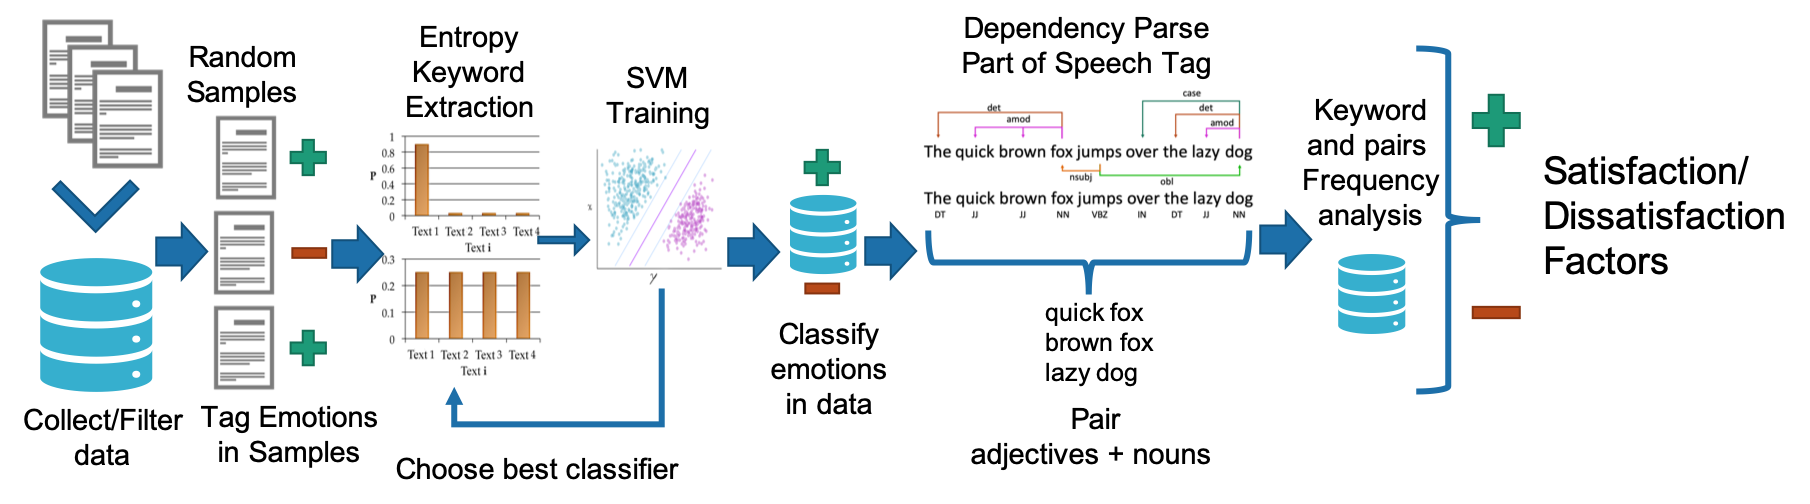
\includegraphics[width=\textwidth]{emotion-method-overview_V3.png}
  \caption{Overview of the methodology to quantitatively rank satisfaction factors.}
  \label{fig:method-overview}
  \end{figure}

  \subsection{Data collection}\label{datacollection}

    In the data collection stage for Chinese reviews in \textit{Ctrip}, a total of \num[group-separator={,}]{5774} review pages of hotels in Japan were collected. From these pages, we extracted a total of \num[group-separator={,}]{245919} reviews, from which \num[group-separator={,}]{211932} were detected to be standard Mandarin Chinese from mainland China. Since a single review can have sentences with different sentiments, we separated sentences using punctuation marks. The Chinese reviews were comprised of \num[group-separator={,}]{187348} separate sentences. 

    In the \textit{TripAdvisor} data collection, we collected data from \num[group-separator={,}]{21380} different hotels. In total, we collected \num[group-separator={,}]{295931} reviews, from which \num[group-separator={,}]{295503} were detected to be in English. Similarly to the Chinese data, we then separated these English reviews into \num[group-separator={,}]{2694261} sentences using the \textit{gensim} python library. For the language detection in both cases we used the \textit{langdetect} python library.

    However, we needed to make the data and comparisons we draw from each of these datasets fair. For that purpose, we filtered both databases only to contain reviews from hotels in both datasets, using their English names to do a search match. We also filtered them to be in the same date range and cut off reviews outside of each other's date ranges. In addition, we selected only the hotels that had a pricing information available. We extracted the lowest price possible for a room or bed for one night, and the highest price possible for one night as well. The difference in pricing can be from better room settings, such as double or twin rooms, or suites of several classes depending on the hotel. Regardless of the reason, the highest priced room can be an indicator of the class of hotel indirectly, which can give us an insight into the kind of service that is offered. After filtering, we found that the number of hotels in common in the data collected was \num[group-separator={,}]{557}. The overlapping date range for reviews was from July 2014 to July 2017. Within these hotels, from \textit{Ctrip} there was \num[group-separator={,}]{48070} reviews comprised of \num[group-separator={,}]{101963} sentences, and from \textit{TripAdvisor} there was \num[group-separator={,}]{41137} reviews comprised of \num[group-separator={,}]{348039} sentences. We found that after filtering the data, the number of reviews was similar for both English and Chinese reviews, but that English reviews tend to be longer in general.

    The price for a night in these hotels ranges from low priced capsule hotels at 2000 yen per night, to high-end hotels \num[group-separator={,}]{188000} yen a night as the far ends of the bell curve. Customers' expectations can vary greatly depending on the pricing of the hotel room they stay at. We therefore made observations on the distribution of pricing in the hotels of our database and binned the data by price ranges, decided by consideration of objective of stay. We show these distributions in Figure \ref{fig:price_dist}. The structure of the data after division by price is shown in Table \ref{tab:exp_notes}, which also includes the results of emotional classification after application of our SVC, as explained in \ref{sentimentanalysis}. 

    \begin{figure}[h]
        \centering
        \begin{subfigure}[b]{0.45\textwidth}
            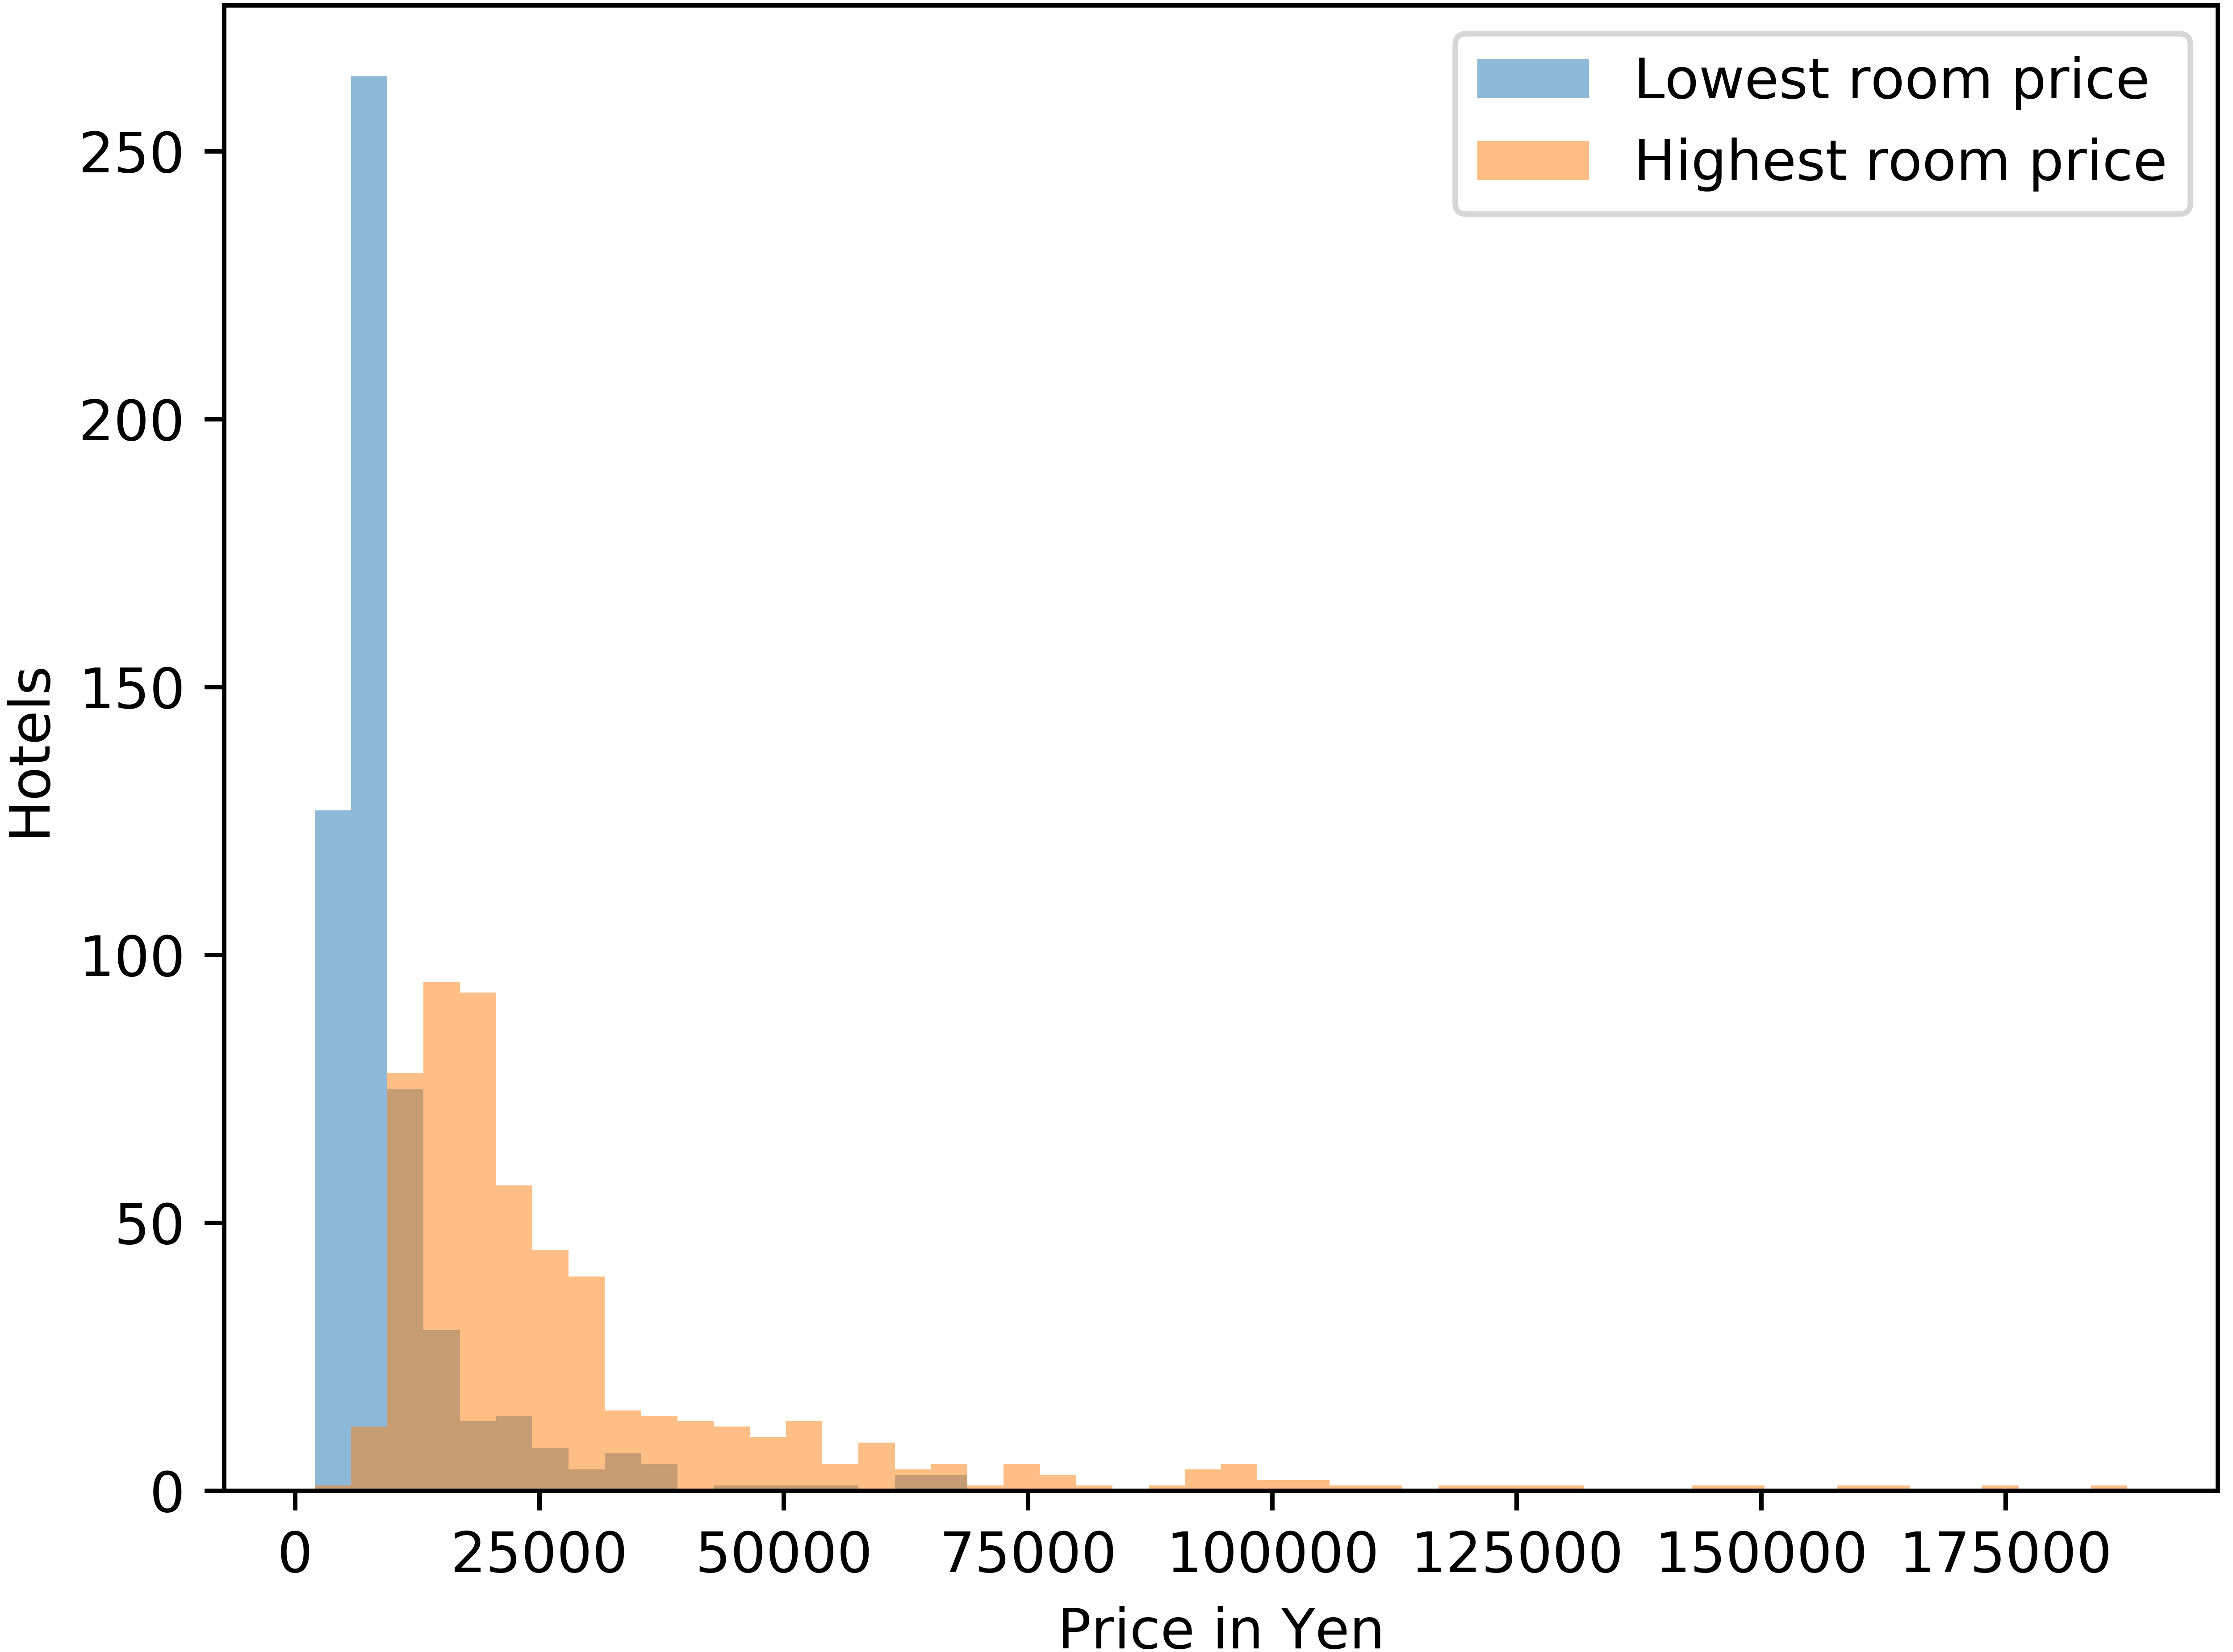
\includegraphics[width=\textwidth]{price_range_distribution_50_even_bins.png}
            \caption{50 equal lenght bins}
        \end{subfigure}
        \begin{subfigure}[b]{0.45\textwidth}
            \includegraphics[width=\textwidth]{price_range_distribution_bins_ver_2.png}
            \caption{manually set 9 price ranges}
        \end{subfigure}
    \caption{Price for one night distribution, blue: lowest price, orange: highest price.}
    \label{fig:price_dist}
    \end{figure}

    % Please add the following required packages to your document preamble:
    % \usepackage{multirow}
    % \usepackage{graphicx}
    \begin{table}[ht]
      \centering
      \caption{Collected data and structure after price range categorizing.}
      \label{tab:exp_notes}
      \resizebox{\textwidth}{!}{%
      \begin{tabular}{|l|l|r|r|}
        \hline
        \multicolumn{1}{|c|}{\textbf{Price range}} & \multicolumn{1}{c|}{\textbf{Data collected}} & \textbf{Ctrip database} & \textbf{Tripadvisor database} \\ \hline
        \multirow{5}{*}{0: All Prices}               & Hotels             & 557     & 557     \\
                                                   & Reviews            & 48,070  & 41,137  \\
                                                   & Sentences          & 101,963 & 348,039 \\
                                                   & Positive sentences & 88,543  & 165,308 \\
                                                   & Negative sentences & 13,420  & 182,731 \\ \hline
        \multirow{2}{*}{1: 0 to 2500 yen}            & Hotels             & 0       & 0       \\
                                                   & Reviews            & 0       & 0       \\ \hline
        \multirow{2}{*}{2: 2500 to 5000 yen}         & Hotels             & 0       & 0       \\
                                                   & Reviews            & 0       & 0       \\ \hline
        \multirow{5}{*}{3: 5000 to 10,000 yen}       & Hotels             & 22      & 22      \\
                                                   & Reviews            & 452     & 459     \\
                                                   & Sentences          & 1,108   & 3,988   \\
                                                   & Positive sentences & 924     & 1,875   \\
                                                   & Negative sentences & 184     & 2,113   \\ \hline
        \multirow{5}{*}{4: 10,000 to 15,000 yen}     & Hotels             & 112     & 112     \\
                                                   & Reviews            & 2,176   & 2,865   \\
                                                   & Sentences          & 4,240   & 24,107  \\
                                                   & Positive sentences & 3,566   & 11,619  \\
                                                   & Negative sentences & 674     & 12,488  \\ \hline
        \multirow{5}{*}{5: 15,000 to 20,000 yen}     & Hotels             & 138     & 138     \\
                                                   & Reviews            & 7,043   & 4,384   \\
                                                   & Sentences          & 14,726  & 37,342  \\
                                                   & Positive sentences & 12,775  & 17,449  \\
                                                   & Negative sentences & 1,951   & 19,893  \\ \hline
        \multirow{5}{*}{6: 20,000 to 30,000 yen}     & Hotels             & 129     & 129     \\
                                                   & Reviews            & 11,845  & 13,772  \\
                                                   & Sentences          & 24,413  & 115,830 \\
                                                   & Positive sentences & 21,068  & 55,381  \\
                                                   & Negative sentences & 3,345   & 60,449  \\ \hline
        \multirow{5}{*}{7: 30,000 to 50,000 yen}     & Hotels             & 83      & 83      \\
                                                   & Reviews            & 8,283   & 7,001   \\
                                                   & Sentences          & 17,939  & 58,409  \\
                                                   & Positive sentences & 15,642  & 28,493  \\
                                                   & Negative sentences & 2,297   & 29,916  \\ \hline
        \multirow{5}{*}{8: 50,000 to 100,000 yen}    & Hotels             & 59      & 59      \\
                                                   & Reviews            & 16,670  & 9,646   \\
                                                   & Sentences          & 36,255  & 81,940  \\
                                                   & Positive sentences & 31,638  & 38,217  \\
                                                   & Negative sentences & 4,617   & 43,723  \\ \hline
        \multirow{5}{*}{9: 100,000 to 200,000 yen}   & Hotels             & 14      & 14      \\
                                                   & Reviews            & 1,601   & 3,010   \\
                                                   & Sentences          & 3,282   & 26,423  \\
                                                   & Positive sentences & 2,930   & 12,274  \\
                                                   & Negative sentences & 352     & 14,149  \\ \hline
        \end{tabular}%
      }
    \end{table}
  \subsection{Text processing}\label{textprocessing}

    Chinese text, unlike English, does not have spaces between each word to separate them. In addition, we also needed to analyze the grammatical relationship between words, be it English or Chinese, in order to understand connections between adjectives and the noun they refer to. For all these processes we used the Stanford CoreNLP pipeline developed by the Natural Language Processing Group at Stanford University \cite[][]{manning-EtAl:2014:P14-5}. In order to separate Chinese words for analysis, we used the Stanford Word Segmenter \cite[][]{chang2008}. In the case of texts in English, however, only using spaces is not enough to correctly collect concepts. The English language is full of variations and conjugations of words depending on the context and tense. Thus, a better segmentation is achieved by using lemmatization, which returns the dictionary form of each word. For this purpose, we used the \textit{gensim} library with the English texts.

    A dependency parser analyzes the grammatical structure of a sentence, detecting connections between words and describing the action and direction of those connections. We show an example of these dependencies in Figure \ref{fig:depparse}. In this study we use the Stanford NLP Dependency Parser, as described in \cite{chen-EMNLP:2014}. A list of dependencies used by this parser is detailed in \cite{marneffe_manning_2016_depparse_manual}. In our study, this step was necessary to extract adjective modifiers and their subject. We did that by parsing the entire database, and extracting instances of a few determined dependency codes. One of these dependency codes is `amod', which stands for adjectival modifier, where an adjective modifies a noun directly (e.g. A big apple). The other dependency code we used was `nsubj', or nominal subject, which is the syntactic subject of a class. We used this one for cases where the adjective is modifying the noun indirectly through other words (e.g. The apple is big). This dependency does not necessarily only include a combination of adjectives and nouns, but it can also be connected with copular verbs, nouns, or other adjectives. For this reason we saw necessary to also perform a Part of Speech (POS) tagging of these clauses.

    \begin{figure}[h]
    \centering
    \includegraphics[width=\textwidth]{depparse.png}
    \caption{Example of dependency parsing.}
    \label{fig:depparse}
    \end{figure}

    A Part of Speech (POS) tagger is a program that assigns word tokens with tags identifying the part of speech. An example is shown in Figure \ref{fig:postag}. A Part of Speech is a category of lexical items that serve similar grammatical purposes; for example, nouns, adjectives, verbs, conjunctions, and so on. In our study, we used the Stanford NLP POS tagger software, described in \cite{toutanova2000enriching, toutanova2003feature}, which uses the Penn Chinese Treebank tags \cite[][]{xia_penntreebank}.  

    \begin{figure}[h]
    \centering
    
\includegraphics[width=\textwidth]{postag.png}
    \caption{Example of POS tagging with the Penn Treebank tags.}
    \label{fig:postag}
    \end{figure}

    In this study we were interested in identifying combinations of adjectives, some verbs and nouns. We also needed to filter away bad combinations that were brought by the versatility of nominal subject dependencies. For this purpose, we identified the tags for nouns, verbs, and adjectives in Chinese and English, with the English tags being a bit more varied. What would be called adjectives in English corresponds more to stative verbs in Chinese, so we needed to extract those as well. We show a detailed description of the chosen tags in Table \ref{tab:target_postag}. We also show a detailed description of the tags we needed to filter, which we selected heuristically by observing commonly found undesired pairs, in Table \ref{tab:filter_postag}.

    % Please add the following required packages to your document preamble:
    % \usepackage{multirow}
    \begin{table}[ht]
      \centering
      \caption{Target Parts of Speech for extraction and pairing.}
      \label{tab:target_postag}
      \begin{tabular}{|c|c|l|l|}
        \hline
        \textbf{Language}                    & \textbf{POS Tag} & \multicolumn{1}{c|}{\textbf{Part of Speech}} & \multicolumn{1}{c|}{\textbf{Examples}}     \\ \hline
        \multirow{4}{*}{Chinese target tags} & NN               & Noun (general)                               & \begin{CJK}{UTF8}{gbsn}酒店\end{CJK} (hotel) \\ \cline{2-4} 
                                             & VA  & Predicative Adjective (verb)       & \begin{CJK}{UTF8}{gbsn}干净 的\end{CJK} (clean)   \\ \cline{2-4} 
                                             & JJ  & Noun modifier (adjectives)         & \begin{CJK}{UTF8}{gbsn}干净\end{CJK} (clean)     \\ \cline{2-4} 
                                             & VV  & Verb (general)                     & \begin{CJK}{UTF8}{gbsn}推荐\end{CJK} (recommend) \\ \hline
        \multirow{9}{*}{English target tags} & NN  & Noun (general)                     & room                                           \\ \cline{2-4} 
                                             & NNS & Noun (plural)                      & beds                                           \\ \cline{2-4} 
                                             & JJ  & Adjective                          & big                                            \\ \cline{2-4} 
                                             & JJS & Adjective (superlative)            & best                                           \\ \cline{2-4} 
                                             & JJR & Adjective (comparative)            & larger                                         \\ \cline{2-4} 
                                             & VB  & Verb (base form)                   & take                                           \\ \cline{2-4} 
                                             & VBP & Verb (single present)              & take                                           \\ \cline{2-4} 
                                             & VBN & Verb (past participle)             & taken                                          \\ \cline{2-4} 
                                             & VBG & Verb (gerund / present participle) & taking                                         \\ \hline
      \end{tabular}
    \end{table}

    % Please add the following required packages to your document preamble:
    % \usepackage{multirow}
    \begin{table}[ht]
      \centering
      \caption{Filtered out Parts of Speech to aid pairing.}
      \label{tab:filter_postag}
      \begin{tabular}{|c|l|l|l|}
        \hline
        \textbf{Language} &
          \multicolumn{1}{c|}{\textbf{POS Tag}} &
          \multicolumn{1}{c|}{\textbf{Part of Speech}} &
          \multicolumn{1}{c|}{\textbf{Examples}} \\ \hline
        \multirow{4}{*}{Commonly filtered tags} & DT    & Determiner         & a, an                                      \\ \cline{2-4} 
                                                & PN    & Pronoun            & I, you, they                               \\ \cline{2-4} 
                                                & CD    & Cardinal Number    & 1, 2, 3, 4, 5                              \\ \cline{2-4} 
                                                & PU    & Punctuation        & .!?                                        \\ \hline
        \multirow{5}{*}{Chinese filtered tags} &
          DEV &
          Particle &
          \begin{CJK}{UTF8}{gbsn}地\end{CJK} (Japan) (adverbial particle) \\ \cline{2-4} 
                                                & NR    & Noun (proper noun) & \begin{CJK}{UTF8}{gbsn}日本\end{CJK} (Japan) \\ \cline{2-4} 
         &
          M &
          Measure word &
          \begin{CJK}{UTF8}{gbsn}个\end{CJK} (general classifier), \begin{CJK}{UTF8}{gbsn}公里\end{CJK} (kilometer) \\ \cline{2-4} 
         &
          SP &
          Sentence-final particle &
          \begin{CJK}{UTF8}{gbsn}他\end{CJK} (he), \begin{CJK}{UTF8}{gbsn}好\end{CJK} (good) \\ \cline{2-4} 
                                                & IJ    & Interjection       & \begin{CJK}{UTF8}{gbsn}啊\end{CJK} (ah)     \\ \hline
        \multirow{3}{*}{English target tags}    & NNP   & Noun (proper noun) & Japan                                      \\ \cline{2-4} 
                                                & PRP\$ & Possessive Pronoun & My, your, her, his                         \\ \cline{2-4} 
                                                & WP    & Wh-pronoun         & What, who                                  \\ \hline
      \end{tabular}
    \end{table}

    Once we had these adjective + noun or verb + noun pairs, we could determine what the customers are referring to in their reviews, and with what frequency they use those pairings positively or negatively.

  \subsection{Sentiment analysis}\label{sentimentanalysis}

    The sentiment analysis was performed using the methodology described in \cite{Aleman2018ICAROB}. Keywords are determined by a comparison of Shannon's entropy \cite[][]{shannon1948} between two classes by a factor of \(\alpha\) for one class and \(\alpha'\) for the other, and then they are used in an SVM \cite[][]{cortes1995}, optimizing keywords to select the best performing classifier using the \(F_1\)-measure \cite{powers2011}. The selected SVM keywords would then clearly represent the user driving factors leading to positive and negative emotions. We also performed experiments to choose the best value of the parameter C used in the SVM. C is a constant that affects the optimization process when minimizing the error of the separating hyperplane. Low values of C give some freedom of error, which minimizes false positives. However, depending on the data, it can increase false negatives. Inversely, high values of C will likely result in minimal false negatives, but a possibility of false positives. SVM performance results are displayed in  Tables \ref{tab:svm_f1_zh} and \ref{tab:svm_f1_en}. Examples of tagged sentences are shown in Table \ref{tab:training_examples}. 

    % Please add the following required packages to your document preamble:
    % \usepackage{graphicx}
    \begin{table}[ht]
      \centering
      \caption{Best performing SVC 5-fold cross-validation Chinese text classifiers.}
      \label{tab:svm_f1_zh}
      % \resizebox{\textwidth}{!}{%
      \begin{tabular}{|l|l|l|l|l|}
        \hline
        \textbf{Keyword List} &
          \textbf{\begin{tabular}[c]{@{}l@{}}Classifier\\ emotion\end{tabular}} &
          \textbf{C} &
          \begin{tabular}[c]{@{}l@{}}\(F_1\)\\ \(\mu\)\end{tabular} &
          \begin{tabular}[c]{@{}l@{}}\(F_1\)\\ \(\sigma\)\end{tabular} \\ \hline
        \begin{tabular}[c]{@{}l@{}}Satisfaction keywords\\ (\(\alpha = 2.75\))\end{tabular} 
                & Satisfaction              & 2.5             & 0.91              & 0.01          \\ \hline
        \begin{tabular}[c]{@{}l@{}}Negative keywords\\ (\(\alpha' = 3.75\))\end{tabular}    
                & Dissatisfaction           & 0.5             & 0.67              & 0.11          \\ \hline
        \begin{tabular}[c]{@{}l@{}}\textbf{Combined}\\ (\(\alpha=2.75\), \(\alpha'=3.75\))\end{tabular} 
                & \textbf{Satisfaction}     & \textbf{0.5}    & \textbf{0.95}     & \textbf{0.01} \\ \hline
        \end{tabular}
        %
        % }
    \end{table}

    % Please add the following required packages to your document preamble:
    % \usepackage{graphicx}
    \begin{table}[ht]
      \centering
      \caption{Best performing SVC 10-fold cross-validation English text classifiers.}
      \label{tab:svm_f1_en}
      % \resizebox{\textwidth}{!}{%
      \begin{tabular}{|l|l|l|l|l|}
        \hline
        \textbf{Keyword List} &
          \textbf{\begin{tabular}[c]{@{}l@{}}Classifier\\ emotion\end{tabular}} &
          \textbf{C} &
          \begin{tabular}[c]{@{}l@{}}\(F_1\)\\ \(\mu\)\end{tabular} &
          \begin{tabular}[c]{@{}l@{}}\(F_1\)\\ \(\sigma\)\end{tabular} \\ \hline
        \begin{tabular}[c]{@{}l@{}}Satisfaction keywords \\ (\(\alpha=1.5\))\end{tabular}       
                & Satisfaction              & 1.75            & 0.82              & 0.02          \\ \hline
        \begin{tabular}[c]{@{}l@{}}Dissatisfaction keywords \\ (\(\alpha'=4.25\))\end{tabular}  
                & Dissatisfaction           & 3               & 0.80              & 0.03          \\ \hline
        \begin{tabular}[c]{@{}l@{}}\textbf{Combined} \\ (\(\alpha=1.5\), \(\alpha'=4.25\))\end{tabular} 
                & \textbf{Satisfaction}     & \textbf{2}      & \textbf{0.83}     & \textbf{0.02} \\ \hline
        \end{tabular}
        %
        % }
    \end{table}

    % Please add the following required packages to your document preamble:
    % \usepackage{multirow}
    % \usepackage{graphicx}
    % \usepackage[normalem]{ulem}
    % \useunder{\uline}{\ul}{}
    \begin{table}[ht]
      \centering
      \caption{Examples of positive and negative sentences used for training SVM.}
      \label{tab:training_examples}
      \resizebox{\textwidth}{!}{%
      \begin{tabular}{|c|c|l|}
        \hline
        \multicolumn{1}{|l|}{\textbf{Language}} &
          \multicolumn{1}{l|}{\textbf{Emotion}} &
          \textbf{Sentences} \\ \hline
        \multirow{4}{*}{Chinese} &
          \multirow{2}{*}{Positive} &
          \begin{tabular}[c]{@{}l@{}}\begin{CJK}{UTF8}{gbsn}酒店 的 服务 很 好 和 我 住 过 的 所有 日本 酒店 一样 各 种 隐形 服务 非常 厉害\end{CJK}\\ (translated as: "The service of the hotel is very good.\\ All the services of the Japanese hotels I have stayed in are extremely good.")\end{tabular} \\ \cline{3-3} 
         &
           &
          \begin{tabular}[c]{@{}l@{}}\begin{CJK}{UTF8}{gbsn}有 一 个 后门 到 地铁站 非常 近 周边 也 算 方便 酒店 服务 和 卫生 都 很 好\end{CJK}\\ (translated as: "There is a back door to the subway station very close to it. \\ The surrounding area is also convenient hotel service and health are very good")\end{tabular} \\ \cline{2-3} 
         &
          \multirow{2}{*}{Negative} &
          \begin{tabular}[c]{@{}l@{}}\begin{CJK}{UTF8}{gbsn}酒店 旁边 很 荒凉 连个 便利 店 都 要 走 很远\end{CJK}\\ (translated as: "The hotel is very bleak, \\ and you have to go very far to go to the nearest convenience store.")\end{tabular} \\ \cline{3-3} 
         &
           &
          \begin{tabular}[c]{@{}l@{}}\begin{CJK}{UTF8}{gbsn}唯一 不 足 是 价格 太高\end{CJK}\\ (translated as: "The only negative is that the price is too high.")\end{tabular} \\ \hline
        \multirow{4}{*}{English} &
          \multirow{2}{*}{Positive} &
          It was extremely clean, peaceful and the hotel Hosts made us feel super welcome \\ \cline{3-3} 
         &
           &
          \begin{tabular}[c]{@{}l@{}}Location is very good, close to a main road with a subway station, a bakery,\\  a 7 eleven and a nice restaurant that is not too expensive but serves good food\end{tabular} \\ \cline{2-3} 
         &
          \multirow{2}{*}{Negative} &
          \begin{tabular}[c]{@{}l@{}}The only downside. Our room was labeled 'non-smoking'\\ but our duvet reeked of smoke.\end{tabular} \\ \cline{3-3} 
         &
           &
          A bit pricey though \\ \hline
        \end{tabular}%
        }
    \end{table}

    Shannon’s entropy can be used to observe the probability distribution of each word inside the corpus. A word that is included in many documents will have a high entropy value for that set of documents. Opposite to this, a word appearing in only one document will have an entropy value of zero. 

    An SVM is trained to classify data based on previously labeled data, generalizing features of the data by defining a separating (p-1)-dimensional hyperplane in a p-dimensional space in which each dimension is a feature of the data. The separating hyperplane, along with the support vectors, divides the multi-dimensional space and minimizes the error of classification. 

    In our study, we used the linear kernel of the SVM classification process, defined by the formula (\ref{eq:svm1}) below. Each training sentence is a point of data, a row in the vector \(x\). Each column represents a feature; in our case, the quantities of each of the keywords in that particular sentence. The labels of previously known classifications (1 for positive, 0 for negative) for each sentence comprise the \(f(x)\) vector. The Weight Vector \(w\) is comprised of the influences each point has had in the training process to define the angle of the hyperplane. The bias coefficient \(b\) determines its position.

    During the SVM learning algorithm, each data point that is classified incorrectly causes a change in the weight vector to classify new data correctly. These changes to the weight vector are greater for features close to the separating hyperplane. These features have stronger changes because they needed to be taken into account to classify with a minimal error. Sequentially, the weight vector can be interpreted as a numerical representation of each feature's effect on each class in the classification process. Below we show the formula for the weight vector \(w\) (\ref{eq:svm_weight}), where \(x\) is the training data and each vectorized sentence \(x_i\) in the data is labeled \(y_i\). Each cycle of the algorithm alters the value of \(w\) by \(\alpha\) to reduce the number of wrong classifications. This equation shows the last value of \(\alpha\) after the end of the cycle.

    \begin{equation}\label{eq:svm1}
    f(x) = w^\top x + b
    \end{equation}

    \begin{equation}\label{eq:svm_weight}
    w = \sum_{i=1}^N \alpha_i y_i x_i
    \end{equation}

    We tagged 159 Chinese sentences and \num[group-separator={,}]{2357} English sentences as positive or negative for our training data. The entropy comparison factors \(\alpha\) and \(\alpha'\) were tested from 1.25 to 6 in intervals of 0.25. We applied this SVC to classify the rest of our data collected. Subsequently, the positive and negative sentences counts shown in Table \ref{tab:exp_notes} are the result of applying our SVC for classification.

\section{Data Analysis}\label{dataanalysis}

  \subsection{Frequent keywords in differently priced hotels}\label{svmresults}

    To understand the satisfaction and dissatisfaction factors of Chinese tourists and English-speaking tourists when lodging in Japan, we study both the frequency of the words they use. Following that, to know the relevance of a keyword as a preference for each group, we observed the frequencies of each entropy-based keyword in our complete data set and in each price range subsequently. The frequency of the keywords in the database shows the level of priority it has for customers.

    We observed the top 10 words with the highest frequencies for keywords that were linked by entropy to satisfaction and dissatisfaction in emotionally positive and negative statements to study. The keywords are the quantitative rank of the needs of Chinese and English speaking customers. We show the top 10 positive keywords for each price range comparing English and Chinese in Table \ref{tab:freq_res_pos}. For the negative keywords, we show the results in Table \ref{tab:freq_res_neg}

  \subsection{Frequently used adjectives and their pairs}\label{adjresults}

    %%%%%%%%%%%%% POSITIVE CHINESE ADJECTIVE PAIRS
    % Please add the following required packages to your document preamble:
    % \usepackage{multirow}
    % \usepackage{graphicx}
    % \usepackage{lscape}
    \begin{landscape}
    \begin{table}[p]
      \centering
      \caption{Top 4 words related to the mainly used adjectives in positive texts.}
      \label{tab:adj_zh_pos}
      \resizebox{\linewidth}{!}{%
      \begin{tabular}{|c|l|l|l|l|l|}
        \hline
        \multicolumn{1}{|l|}{\textbf{Price range}} &
          \multicolumn{1}{c|}{\textbf{\begin{CJK}{UTF8}{gbsn}不错\end{CJK} (not bad)}} &
          \multicolumn{1}{c|}{\textbf{\begin{CJK}{UTF8}{gbsn}大\end{CJK} (big)}} &
          \multicolumn{1}{c|}{\textbf{\begin{CJK}{UTF8}{gbsn}干净\end{CJK} (clean)}} &
          \multicolumn{1}{c|}{\textbf{\begin{CJK}{UTF8}{gbsn}近\end{CJK} (near)}} &
          \multicolumn{1}{c|}{\textbf{\begin{CJK}{UTF8}{gbsn}新\end{CJK} (new)}} \\ \hline
        \multirow{5}{*}{\textbf{0: All Prices}} &
          \begin{CJK}{UTF8}{gbsn}不错\end{CJK} (not bad) : 12892 &
          \begin{CJK}{UTF8}{gbsn}大\end{CJK} (big) : 9844 &
          \begin{CJK}{UTF8}{gbsn}干净\end{CJK} (clean) : 6665 &
          \begin{CJK}{UTF8}{gbsn}近\end{CJK} (near) : 5181 &
          \begin{CJK}{UTF8}{gbsn}新\end{CJK} (new) : 2775 \\
         &
          \begin{CJK}{UTF8}{gbsn}不错 酒店\end{CJK} (nice hotel) : 1462 &
          \begin{CJK}{UTF8}{gbsn}大 房间\end{CJK} (big room) : 3197 &
          \begin{CJK}{UTF8}{gbsn}干净 房间\end{CJK} (clean room) : 1224 &
          \begin{CJK}{UTF8}{gbsn}近 酒店\end{CJK} (near hotel) : 453 &
          \begin{CJK}{UTF8}{gbsn}新 设施\end{CJK} (new facility) : 363 \\
         &
          \begin{CJK}{UTF8}{gbsn}不错 位置\end{CJK} (nice location) : 1426 &
          \begin{CJK}{UTF8}{gbsn}大 床\end{CJK} (big bed) : 772 &
          \begin{CJK}{UTF8}{gbsn}干净 酒店\end{CJK} (clean hotel) : 737 &
          \begin{CJK}{UTF8}{gbsn}近 桥\end{CJK} (near bridge) : 144 &
          \begin{CJK}{UTF8}{gbsn}新 酒店\end{CJK} (new hotel) : 246 \\
         &
          \begin{CJK}{UTF8}{gbsn}不错 服务\end{CJK} (nice service) : 869 &
          \begin{CJK}{UTF8}{gbsn}大 酒店\end{CJK} (big hotel) : 379 &
          \begin{CJK}{UTF8}{gbsn}干净 卫生\end{CJK} (clean and hygienic) : 464 &
          \begin{CJK}{UTF8}{gbsn}近 地铁站\end{CJK} (near subway station) : 122 &
          \begin{CJK}{UTF8}{gbsn}新 装修\end{CJK} (new decoration) : 116 \\
         &
          \begin{CJK}{UTF8}{gbsn}不错 环境\end{CJK} (nice environment) : 714 &
          \begin{CJK}{UTF8}{gbsn}大 超市\end{CJK} (big supermarket) : 232 &
          \begin{CJK}{UTF8}{gbsn}干净 环境\end{CJK} (clean environment) : 61 &
          \begin{CJK}{UTF8}{gbsn}近 站\end{CJK} (near station) : 108 &
          \begin{CJK}{UTF8}{gbsn}新 房间\end{CJK} (new room) : 53 \\ \hline
        \multirow{5}{*}{\textbf{3: 5000 to 10,000 yen}} &
          \begin{CJK}{UTF8}{gbsn}不错\end{CJK} (not bad) : 139 &
          \begin{CJK}{UTF8}{gbsn}大\end{CJK} (big) : 76 &
          \begin{CJK}{UTF8}{gbsn}干净\end{CJK} (clean) : 114 &
          \begin{CJK}{UTF8}{gbsn}近\end{CJK} (near) : 55 &
           \\
         &
          \begin{CJK}{UTF8}{gbsn}不错 酒店\end{CJK} (nice hotel) : 17 &
          \begin{CJK}{UTF8}{gbsn}大 房间\end{CJK} (big room) : 11 &
          \begin{CJK}{UTF8}{gbsn}干净 房间\end{CJK} (clean room) : 21 &
          \begin{CJK}{UTF8}{gbsn}近 酒店\end{CJK} (near hotel) : 4 &
           \\
         &
          \begin{CJK}{UTF8}{gbsn}不错 位置\end{CJK} (nice location) : 16 &
          \begin{CJK}{UTF8}{gbsn}大 床\end{CJK} (big bed) : 10 &
          \begin{CJK}{UTF8}{gbsn}干净 酒店\end{CJK} (clean hotel) : 10 &
          \begin{CJK}{UTF8}{gbsn}近 地铁\end{CJK} (near subway) : 2 &
           \\
         &
          \begin{CJK}{UTF8}{gbsn}不错 早餐\end{CJK} (nice breakfast) : 12 &
          \begin{CJK}{UTF8}{gbsn}大 超市\end{CJK} (big supermarket) : 5 &
          \begin{CJK}{UTF8}{gbsn}干净 卫生\end{CJK} (clean and hygienic) : 6 &
          \begin{CJK}{UTF8}{gbsn}不错 附近\end{CJK} (not bad nearby) : 0 &
           \\
         &
          \begin{CJK}{UTF8}{gbsn}不错 服务\end{CJK} (nice service) : 8 &
          \begin{CJK}{UTF8}{gbsn}大 商场\end{CJK} (big market) : 3 &
          \begin{CJK}{UTF8}{gbsn}干净 总体\end{CJK} (clean overall) : 4 &
          \begin{CJK}{UTF8}{gbsn}便利 附 近\end{CJK} (convenient nearby) : 0 &
           \\ \hline
        \multirow{5}{*}{\textbf{4: 10,000 to 15,000 yen}} &
          \begin{CJK}{UTF8}{gbsn}不错\end{CJK} (not bad) : 601 &
          \begin{CJK}{UTF8}{gbsn}大\end{CJK} (big) : 348 &
          \begin{CJK}{UTF8}{gbsn}干净\end{CJK} (clean) : 455 &
          \begin{CJK}{UTF8}{gbsn}近\end{CJK} (near) : 323 &
          \begin{CJK}{UTF8}{gbsn}新\end{CJK} (new) : 37 \\
         &
          \begin{CJK}{UTF8}{gbsn}不错 位置\end{CJK} (nice location) : 72 &
          \begin{CJK}{UTF8}{gbsn}大 房间\end{CJK} (big room) : 76 &
          \begin{CJK}{UTF8}{gbsn}干净 房间\end{CJK} (clean room) : 66 &
          \begin{CJK}{UTF8}{gbsn}近 酒店\end{CJK} (near hotel) : 27 &
          \begin{CJK}{UTF8}{gbsn}新 设施\end{CJK} (new facility) : 9 \\
         &
          \begin{CJK}{UTF8}{gbsn}不错 酒店\end{CJK} (nice hotel) : 37 &
          \begin{CJK}{UTF8}{gbsn}大 床\end{CJK} (big bed) : 30 &
          \begin{CJK}{UTF8}{gbsn}干净 卫生\end{CJK} (clean and hygienic) : 52 &
          \begin{CJK}{UTF8}{gbsn}近 站\end{CJK} (near station) : 14 &
          \begin{CJK}{UTF8}{gbsn}新 装修\end{CJK} (new decoration) : 2 \\
         &
          \begin{CJK}{UTF8}{gbsn}不错 服务\end{CJK} (nice service) : 34 &
          \begin{CJK}{UTF8}{gbsn}大 社\end{CJK} (big club) : 26 &
          \begin{CJK}{UTF8}{gbsn}干净 酒店\end{CJK} (clean hotel) : 48 &
          \begin{CJK}{UTF8}{gbsn}近 地铁\end{CJK} (near subway) : 12 &
          \begin{CJK}{UTF8}{gbsn}新 酒店\end{CJK} (new hotel) : 2 \\
         &
          \begin{CJK}{UTF8}{gbsn}不错 早餐\end{CJK} (nice breakfast) : 26 &
          \begin{CJK}{UTF8}{gbsn}大 空间\end{CJK} (big space) : 16 &
          \begin{CJK}{UTF8}{gbsn}干净 打扫\end{CJK} (clean up) : 9 &
          \begin{CJK}{UTF8}{gbsn}近 车站\end{CJK} (near the station) : 10 &
           \\ \hline
        \multirow{5}{*}{\textbf{5: 15,000 to 20,000 yen}} &
          \begin{CJK}{UTF8}{gbsn}不错\end{CJK} (not bad) : 1925 &
          \begin{CJK}{UTF8}{gbsn}大\end{CJK} (big) : 1277 &
          \begin{CJK}{UTF8}{gbsn}干净\end{CJK} (clean) : 1348 &
          \begin{CJK}{UTF8}{gbsn}近\end{CJK} (near) : 1016 &
          \begin{CJK}{UTF8}{gbsn}新\end{CJK} (new) : 234 \\
         &
          \begin{CJK}{UTF8}{gbsn}不错 位置\end{CJK} (nice location) : 207 &
          \begin{CJK}{UTF8}{gbsn}大 房间\end{CJK} (big room) : 316 &
          \begin{CJK}{UTF8}{gbsn}干净 房间\end{CJK} (clean room) : 234 &
          \begin{CJK}{UTF8}{gbsn}近 酒店\end{CJK} (near hotel) : 82 &
          \begin{CJK}{UTF8}{gbsn}新 设施\end{CJK} (new facility) : 47 \\
         &
          \begin{CJK}{UTF8}{gbsn}不错 酒店\end{CJK} (nice hotel) : 168 &
          \begin{CJK}{UTF8}{gbsn}大 床\end{CJK} (big bed) : 140 &
          \begin{CJK}{UTF8}{gbsn}干净 酒店\end{CJK} (clean hotel) : 161 &
          \begin{CJK}{UTF8}{gbsn}近 站\end{CJK} (near station) : 35 &
          \begin{CJK}{UTF8}{gbsn}新 酒店\end{CJK} (new hotel) : 25 \\
         &
          \begin{CJK}{UTF8}{gbsn}不错 服务\end{CJK} (nice service) : 131 &
          \begin{CJK}{UTF8}{gbsn}大 超市\end{CJK} (big supermarket) : 73 &
          \begin{CJK}{UTF8}{gbsn}干净 卫生\end{CJK} (clean and hygienic) : 92 &
          \begin{CJK}{UTF8}{gbsn}近 地铁站\end{CJK} (near subway station) : 34 &
          \begin{CJK}{UTF8}{gbsn}新 装修\end{CJK} (new decoration) : 15 \\
         &
          \begin{CJK}{UTF8}{gbsn}不错 早餐\end{CJK} (nice breakfast) : 109 &
          \begin{CJK}{UTF8}{gbsn}大 酒店\end{CJK} (big hotel) : 49 &
          \begin{CJK}{UTF8}{gbsn}干净 设施\end{CJK} (clean facilities) : 19 &
          \begin{CJK}{UTF8}{gbsn}近 桥\end{CJK} (near bridge) : 29 &
          \begin{CJK}{UTF8}{gbsn}新 房间\end{CJK} (new room) : 10 \\ \hline
        \multirow{5}{*}{\textbf{6: 20,000 to 30,000 yen}} &
          \begin{CJK}{UTF8}{gbsn}不错\end{CJK} (not bad) : 3110 &
          \begin{CJK}{UTF8}{gbsn}大\end{CJK} (big) : 2245 &
          \begin{CJK}{UTF8}{gbsn}干净\end{CJK} (clean) : 1940 &
          \begin{CJK}{UTF8}{gbsn}近\end{CJK} (near) : 1433 &
          \begin{CJK}{UTF8}{gbsn}新\end{CJK} (new) : 517 \\
         &
          \begin{CJK}{UTF8}{gbsn}不错 位置\end{CJK} (nice location) : 409 &
          \begin{CJK}{UTF8}{gbsn}大 房间\end{CJK} (big room) : 680 &
          \begin{CJK}{UTF8}{gbsn}干净 房间\end{CJK} (clean room) : 360 &
          \begin{CJK}{UTF8}{gbsn}近 酒店\end{CJK} (near hotel) : 164 &
          \begin{CJK}{UTF8}{gbsn}新 设施\end{CJK} (new facility) : 89 \\
         &
          \begin{CJK}{UTF8}{gbsn}不错 酒店\end{CJK} (nice hotel) : 326 &
          \begin{CJK}{UTF8}{gbsn}大 床\end{CJK} (big bed) : 198 &
          \begin{CJK}{UTF8}{gbsn}干净 酒店\end{CJK} (clean hotel) : 203 &
          \begin{CJK}{UTF8}{gbsn}近 地铁\end{CJK} (near subway) : 34 &
          \begin{CJK}{UTF8}{gbsn}新 酒店\end{CJK} (new hotel) : 51 \\
         &
          \begin{CJK}{UTF8}{gbsn}不错 服务\end{CJK} (nice service) : 206 &
          \begin{CJK}{UTF8}{gbsn}大 酒店\end{CJK} (big hotel) : 102 &
          \begin{CJK}{UTF8}{gbsn}干净 卫生\end{CJK} (clean and hygienic) : 137 &
          \begin{CJK}{UTF8}{gbsn}近 地铁站\end{CJK} (near subway station) : 31 &
          \begin{CJK}{UTF8}{gbsn}新 装修\end{CJK} (new decoration) : 24 \\
         &
          \begin{CJK}{UTF8}{gbsn}不错 环境\end{CJK} (nice environment) : 183 &
          \begin{CJK}{UTF8}{gbsn}大 空间\end{CJK} (big space) : 64 &
          \begin{CJK}{UTF8}{gbsn}干净 环境\end{CJK} (clean environment) : 21 &
          \begin{CJK}{UTF8}{gbsn}近 车站\end{CJK} (near the station) : 27 &
          \begin{CJK}{UTF8}{gbsn}新 房间\end{CJK} (new room) : 10 \\ \hline
        \multirow{5}{*}{\textbf{7: 30,000 to 50,000 yen}} &
          \begin{CJK}{UTF8}{gbsn}不错\end{CJK} (not bad) : 2291 &
          \begin{CJK}{UTF8}{gbsn}大\end{CJK} (big) : 1913 &
          \begin{CJK}{UTF8}{gbsn}干净\end{CJK} (clean) : 1159 &
          \begin{CJK}{UTF8}{gbsn}近\end{CJK} (near) : 935 &
          \begin{CJK}{UTF8}{gbsn}新\end{CJK} (new) : 260 \\
         &
          \begin{CJK}{UTF8}{gbsn}不错 位置\end{CJK} (nice location) : 277 &
          \begin{CJK}{UTF8}{gbsn}大 房间\end{CJK} (big room) : 643 &
          \begin{CJK}{UTF8}{gbsn}干净 房间\end{CJK} (clean room) : 224 &
          \begin{CJK}{UTF8}{gbsn}近 酒店\end{CJK} (near hotel) : 80 &
          \begin{CJK}{UTF8}{gbsn}新 设施\end{CJK} (new facility) : 63 \\
         &
          \begin{CJK}{UTF8}{gbsn}不错 酒店\end{CJK} (nice hotel) : 274 &
          \begin{CJK}{UTF8}{gbsn}大 床\end{CJK} (big bed) : 141 &
          \begin{CJK}{UTF8}{gbsn}干净 酒店\end{CJK} (clean hotel) : 146 &
          \begin{CJK}{UTF8}{gbsn}近 站\end{CJK} (near station) : 24 &
          \begin{CJK}{UTF8}{gbsn}新 酒店\end{CJK} (new hotel) : 25 \\
         &
          \begin{CJK}{UTF8}{gbsn}不错 服务\end{CJK} (nice service) : 140 &
          \begin{CJK}{UTF8}{gbsn}大 超市\end{CJK} (big supermarket) : 74 &
          \begin{CJK}{UTF8}{gbsn}干净 卫生\end{CJK} (clean and hygienic) : 71 &
          \begin{CJK}{UTF8}{gbsn}近 桥\end{CJK} (near bridge) : 20 &
          \begin{CJK}{UTF8}{gbsn}新 装修\end{CJK} (new decoration) : 15 \\
         &
          \begin{CJK}{UTF8}{gbsn}不错 环境\end{CJK} (nice environment) : 140 &
          \begin{CJK}{UTF8}{gbsn}大 酒店\end{CJK} (big hotel) : 66 &
          \begin{CJK}{UTF8}{gbsn}干净 环境\end{CJK} (clean environment) : 16 &
          \begin{CJK}{UTF8}{gbsn}近 山\end{CJK} (near mountain) : 12 &
          \begin{CJK}{UTF8}{gbsn}新 房间\end{CJK} (new room) : 11 \\ \hline
        \multirow{5}{*}{\textbf{8: 50,000 to 100,000}} &
          \begin{CJK}{UTF8}{gbsn}不错\end{CJK} (not bad) : 4451 &
          \begin{CJK}{UTF8}{gbsn}大\end{CJK} (big) : 3670 &
          \begin{CJK}{UTF8}{gbsn}干净\end{CJK} (clean) : 1577 &
          \begin{CJK}{UTF8}{gbsn}近\end{CJK} (near) : 1354 &
          \begin{CJK}{UTF8}{gbsn}新\end{CJK} (new) : 1634 \\
         &
          \begin{CJK}{UTF8}{gbsn}不错 酒店\end{CJK} (nice hotel) : 587 &
          \begin{CJK}{UTF8}{gbsn}大 房间\end{CJK} (big room) : 1340 &
          \begin{CJK}{UTF8}{gbsn}干净 房间\end{CJK} (clean room) : 310 &
          \begin{CJK}{UTF8}{gbsn}近 酒店\end{CJK} (near hotel) : 88 &
          \begin{CJK}{UTF8}{gbsn}新 设施\end{CJK} (new facility) : 141 \\
         &
          \begin{CJK}{UTF8}{gbsn}不错 位置\end{CJK} (nice location) : 415 &
          \begin{CJK}{UTF8}{gbsn}大 床\end{CJK} (big bed) : 238 &
          \begin{CJK}{UTF8}{gbsn}干净 酒店\end{CJK} (clean hotel) : 161 &
          \begin{CJK}{UTF8}{gbsn}近 桥\end{CJK} (near bridge) : 76 &
          \begin{CJK}{UTF8}{gbsn}新 酒店\end{CJK} (new hotel) : 123 \\
         &
          \begin{CJK}{UTF8}{gbsn}不错 服务\end{CJK} (nice service) : 328 &
          \begin{CJK}{UTF8}{gbsn}大 酒店\end{CJK} (big hotel) : 144 &
          \begin{CJK}{UTF8}{gbsn}干净 卫生\end{CJK} (clean and hygienic) : 101 &
          \begin{CJK}{UTF8}{gbsn}近 地铁站\end{CJK} (near subway station) : 35 &
          \begin{CJK}{UTF8}{gbsn}新 装修\end{CJK} (new decoration) : 57 \\
         &
          \begin{CJK}{UTF8}{gbsn}不错 早餐\end{CJK} (nice breakfast) : 251 &
          \begin{CJK}{UTF8}{gbsn}大 商场\end{CJK} (big market) : 88 &
          \begin{CJK}{UTF8}{gbsn}干净 服务\end{CJK} (clean service) : 13 &
          \begin{CJK}{UTF8}{gbsn}近 铁\end{CJK} (Kintetsu) : 24 &
          \begin{CJK}{UTF8}{gbsn}新 斋\end{CJK} (new) : 22 \\ \hline
        \multirow{5}{*}{\textbf{9: 100,000 to 200,000}} &
          \begin{CJK}{UTF8}{gbsn}不错\end{CJK} (not bad) : 375 &
          \begin{CJK}{UTF8}{gbsn}大\end{CJK} (big) : 315 &
          \begin{CJK}{UTF8}{gbsn}干净\end{CJK} (clean) : 72 &
          \begin{CJK}{UTF8}{gbsn}近\end{CJK} (near) : 65 &
          \begin{CJK}{UTF8}{gbsn}新\end{CJK} (new) : 77 \\
         &
          \begin{CJK}{UTF8}{gbsn}不错 酒店\end{CJK} (nice hotel) : 53 &
          \begin{CJK}{UTF8}{gbsn}大 房间\end{CJK} (big room) : 131 &
          \begin{CJK}{UTF8}{gbsn}干净 房间\end{CJK} (clean room) : 9 &
          \begin{CJK}{UTF8}{gbsn}近 酒店\end{CJK} (near hotel) : 8 &
          \begin{CJK}{UTF8}{gbsn}新 酒店\end{CJK} (new hotel) : 19 \\
         &
          \begin{CJK}{UTF8}{gbsn}不错 位置\end{CJK} (nice location) : 30 &
          \begin{CJK}{UTF8}{gbsn}大 面积\end{CJK} (large area) : 19 &
          \begin{CJK}{UTF8}{gbsn}干净 酒店\end{CJK} (clean hotel) : 8 &
          \begin{CJK}{UTF8}{gbsn}近 地铁站\end{CJK} (near subway station) : 3 &
          \begin{CJK}{UTF8}{gbsn}新 设施\end{CJK} (new facility) : 13 \\
         &
          \begin{CJK}{UTF8}{gbsn}不错 环境\end{CJK} (nice environment) : 27 &
          \begin{CJK}{UTF8}{gbsn}大 床\end{CJK} (big bed) : 15 &
          \begin{CJK}{UTF8}{gbsn}干净 卫生\end{CJK} (clean and hygienic) : 5 &
          \begin{CJK}{UTF8}{gbsn}近 市场\end{CJK} (near market) : 3 &
          \begin{CJK}{UTF8}{gbsn}新 装修\end{CJK} (new decoration) : 3 \\
         &
          \begin{CJK}{UTF8}{gbsn}不错 服务\end{CJK} (nice service) : 22 &
          \begin{CJK}{UTF8}{gbsn}大 卫生间\end{CJK} (big toilet) : 13 &
          \begin{CJK}{UTF8}{gbsn}干净 一如既往\end{CJK} (clean as always) : 0 &
          \begin{CJK}{UTF8}{gbsn}不错 附近\end{CJK} (not bad nearby) : 0 &
          \begin{CJK}{UTF8}{gbsn}新 位置\end{CJK} (new location) : 2 \\ \hline
        \end{tabular}%
        }
      \end{table}
    \end{landscape}


    %%%%%%%%%%%%% NEGATIVE CHINESE ADJECTIVE PAIRS
    % Please add the following required packages to your document preamble:
    % \usepackage{multirow}
    % \usepackage{graphicx}
    % \usepackage{lscape}
    \begin{landscape}
    \begin{table}[p]
      \centering
      \caption{Top 4 words related to the mainly used adjectives in negative texts.}
      \label{tab:adj_zh_neg}
      \resizebox{\linewidth}{!}{%
      \begin{tabular}{|c|l|l|l|}
        \hline
        \multicolumn{1}{|l|}{\textbf{Price range}} &
          \multicolumn{1}{c|}{\textbf{\begin{CJK}{UTF8}{gbsn}一般\end{CJK} (general)}} &
          \multicolumn{1}{c|}{\textbf{\begin{CJK}{UTF8}{gbsn}陈旧\end{CJK} (obsolete)}} &
          \multicolumn{1}{c|}{\textbf{\begin{CJK}{UTF8}{gbsn}老\end{CJK} (old)}} \\ \hline
        \multirow{5}{*}{\textbf{0: All Prices}} &
          \begin{CJK}{UTF8}{gbsn}一般\end{CJK} (general) : 1713 &
          \begin{CJK}{UTF8}{gbsn}陈旧\end{CJK} (obsolete) : 319 &
          \begin{CJK}{UTF8}{gbsn}老\end{CJK} (old) : 297 \\
         &
          \begin{CJK}{UTF8}{gbsn}一般 设施\end{CJK} (general facilities) : 137 &
          \begin{CJK}{UTF8}{gbsn}陈旧 设施\end{CJK} (obsolete facilities) : 184 &
          \begin{CJK}{UTF8}{gbsn}老 酒店\end{CJK} (old hotel) : 74 \\
         &
          \begin{CJK}{UTF8}{gbsn}一般 服务\end{CJK} (general service) : 115 &
          \begin{CJK}{UTF8}{gbsn}陈旧 设备\end{CJK} (obsolete equipment) : 18 &
          \begin{CJK}{UTF8}{gbsn}老 设施\end{CJK} (old facility) : 58 \\
         &
          \begin{CJK}{UTF8}{gbsn}一般 酒店\end{CJK} (average hotel) : 106 &
          \begin{CJK}{UTF8}{gbsn}陈旧 房间\end{CJK} (outdated room) : 10 &
          \begin{CJK}{UTF8}{gbsn}老 店\end{CJK} (old shop) : 15 \\
         &
          \begin{CJK}{UTF8}{gbsn}一般 早餐\end{CJK} (average breakfast) : 97 &
          \begin{CJK}{UTF8}{gbsn}陈旧 酒店\end{CJK} (outdated hotel) : 10 &
          \begin{CJK}{UTF8}{gbsn}老 装修\end{CJK} (old decoration) : 11 \\ \hline
        \multirow{5}{*}{\textbf{3: 5000 to 10,000 yen}} &
          \begin{CJK}{UTF8}{gbsn}一般\end{CJK} (general) : 28 &
           &
          \begin{CJK}{UTF8}{gbsn}老\end{CJK} (old) : 2 \\
         &
          \begin{CJK}{UTF8}{gbsn}一般 设施\end{CJK} (general facilities) : 5 &
           &
           \\
         &
          \begin{CJK}{UTF8}{gbsn}一般 早餐\end{CJK} (average breakfast) : 3 &
           &
           \\
         &
          \begin{CJK}{UTF8}{gbsn}一般 味道\end{CJK} (general taste) : 2 &
           &
           \\
         &
          \begin{CJK}{UTF8}{gbsn}一般 效果\end{CJK} (general effect) : 2 &
           &
           \\ \hline
        \multirow{5}{*}{\textbf{4: 10,000 to 15,000 yen}} &
          \begin{CJK}{UTF8}{gbsn}一般\end{CJK} (general) : 91 &
          \begin{CJK}{UTF8}{gbsn}陈旧\end{CJK} (obsolete) : 34 &
          \begin{CJK}{UTF8}{gbsn}老\end{CJK} (old) : 30 \\
         &
          \begin{CJK}{UTF8}{gbsn}一般 设施\end{CJK} (general facilities) : 10 &
          \begin{CJK}{UTF8}{gbsn}陈旧 设施\end{CJK} (obsolete facilities) : 17 &
          \begin{CJK}{UTF8}{gbsn}老 酒店\end{CJK} (old hotel) : 8 \\
         &
          \begin{CJK}{UTF8}{gbsn}一般 位置\end{CJK} (general location) : 8 &
          \begin{CJK}{UTF8}{gbsn}陈旧 家具\end{CJK} (obsolete furniture) : 2 &
          \begin{CJK}{UTF8}{gbsn}老 设施\end{CJK} (old facility) : 7 \\
         &
          \begin{CJK}{UTF8}{gbsn}一般 酒店\end{CJK} (average hotel) : 6 &
          \begin{CJK}{UTF8}{gbsn}陈旧 设备\end{CJK} (obsolete equipment) : 2 &
          \begin{CJK}{UTF8}{gbsn}老 建筑\end{CJK} (old building) : 3 \\
         &
          \begin{CJK}{UTF8}{gbsn}一般 早餐\end{CJK} (average breakfast) : 5 &
           &
           \\ \hline
        \multirow{5}{*}{\textbf{5: 15,000 to 20,000 yen}} &
          \begin{CJK}{UTF8}{gbsn}一般\end{CJK} (general) : 218 &
          \begin{CJK}{UTF8}{gbsn}陈旧\end{CJK} (obsolete) : 43 &
          \begin{CJK}{UTF8}{gbsn}老\end{CJK} (old) : 26 \\
         &
          \begin{CJK}{UTF8}{gbsn}一般 设施\end{CJK} (general facilities) : 23 &
          \begin{CJK}{UTF8}{gbsn}陈旧 设施\end{CJK} (obsolete facilities) : 25 &
          \begin{CJK}{UTF8}{gbsn}老 酒店\end{CJK} (old hotel) : 11 \\
         &
          \begin{CJK}{UTF8}{gbsn}一般 酒店\end{CJK} (average hotel) : 21 &
          \begin{CJK}{UTF8}{gbsn}陈旧 设备\end{CJK} (obsolete equipment) : 3 &
          \begin{CJK}{UTF8}{gbsn}老 设施\end{CJK} (old facility) : 7 \\
         &
          \begin{CJK}{UTF8}{gbsn}一般 早餐\end{CJK} (average breakfast) : 14 &
          \begin{CJK}{UTF8}{gbsn}陈旧 酒店\end{CJK} (outdated hotel) : 2 &
          \begin{CJK}{UTF8}{gbsn}老 外观\end{CJK} (old appearance) : 2 \\
         &
          \begin{CJK}{UTF8}{gbsn}一般 卫生\end{CJK} (general hygiene) : 8 &
           &
           \\ \hline
        \multirow{5}{*}{\textbf{6: 20,000 to 30,000 yen}} &
          \begin{CJK}{UTF8}{gbsn}一般\end{CJK} (general) : 504 &
          \begin{CJK}{UTF8}{gbsn}陈旧\end{CJK} (obsolete) : 75 &
          \begin{CJK}{UTF8}{gbsn}老\end{CJK} (old) : 55 \\
         &
          \begin{CJK}{UTF8}{gbsn}一般 设施\end{CJK} (general facilities) : 42 &
          \begin{CJK}{UTF8}{gbsn}陈旧 设施\end{CJK} (obsolete facilities) : 42 &
          \begin{CJK}{UTF8}{gbsn}老 酒店\end{CJK} (old hotel) : 9 \\
         &
          \begin{CJK}{UTF8}{gbsn}一般 酒店\end{CJK} (average hotel) : 37 &
          \begin{CJK}{UTF8}{gbsn}陈旧 设备\end{CJK} (obsolete equipment) : 7 &
          \begin{CJK}{UTF8}{gbsn}老 设施\end{CJK} (old facility) : 8 \\
         &
          \begin{CJK}{UTF8}{gbsn}一般 服务\end{CJK} (general service) : 34 &
          \begin{CJK}{UTF8}{gbsn}陈旧 装修\end{CJK} (old decoration) : 3 &
          \begin{CJK}{UTF8}{gbsn}老 店\end{CJK} (old shop) : 3 \\
         &
          \begin{CJK}{UTF8}{gbsn}一般 早餐\end{CJK} (average breakfast) : 21 &
          \begin{CJK}{UTF8}{gbsn}陈旧 酒店\end{CJK} (outdated hotel) : 2 &
          \begin{CJK}{UTF8}{gbsn}老 房间\end{CJK} (old room) : 3 \\ \hline
        \multirow{5}{*}{\textbf{7: 30,000 to 50,000 yen}} &
          \begin{CJK}{UTF8}{gbsn}一般\end{CJK} (general) : 311 &
          \begin{CJK}{UTF8}{gbsn}陈旧\end{CJK} (obsolete) : 71 &
          \begin{CJK}{UTF8}{gbsn}老\end{CJK} (old) : 45 \\
         &
          \begin{CJK}{UTF8}{gbsn}一般 设施\end{CJK} (general facilities) : 23 &
          \begin{CJK}{UTF8}{gbsn}陈旧 设施\end{CJK} (obsolete facilities) : 43 &
          \begin{CJK}{UTF8}{gbsn}老 酒店\end{CJK} (old hotel) : 11 \\
         &
          \begin{CJK}{UTF8}{gbsn}一般 服务\end{CJK} (general service) : 22 &
          \begin{CJK}{UTF8}{gbsn}陈旧 设备\end{CJK} (obsolete equipment) : 5 &
          \begin{CJK}{UTF8}{gbsn}老 设施\end{CJK} (old facility) : 7 \\
         &
          \begin{CJK}{UTF8}{gbsn}一般 早餐\end{CJK} (average breakfast) : 19 &
          \begin{CJK}{UTF8}{gbsn}陈旧 房间\end{CJK} (outdated room) : 3 &
          \begin{CJK}{UTF8}{gbsn}老 店\end{CJK} (old shop) : 3 \\
         &
          \begin{CJK}{UTF8}{gbsn}一般 酒店\end{CJK} (average hotel) : 15 &
           &
          \begin{CJK}{UTF8}{gbsn}老 房间\end{CJK} (old room) : 2 \\ \hline
        \multirow{5}{*}{\textbf{8: 50,000 to 100,000}} &
          \begin{CJK}{UTF8}{gbsn}一般\end{CJK} (general) : 510 &
          \begin{CJK}{UTF8}{gbsn}陈旧\end{CJK} (obsolete) : 90 &
          \begin{CJK}{UTF8}{gbsn}老\end{CJK} (old) : 134 \\
         &
          \begin{CJK}{UTF8}{gbsn}一般 服务\end{CJK} (general service) : 39 &
          \begin{CJK}{UTF8}{gbsn}陈旧 设施\end{CJK} (obsolete facilities) : 53 &
          \begin{CJK}{UTF8}{gbsn}老 酒店\end{CJK} (old hotel) : 34 \\
         &
          \begin{CJK}{UTF8}{gbsn}一般 设施\end{CJK} (general facilities) : 32 &
          \begin{CJK}{UTF8}{gbsn}陈旧 房间\end{CJK} (outdated room) : 5 &
          \begin{CJK}{UTF8}{gbsn}老 设施\end{CJK} (old facility) : 26 \\
         &
          \begin{CJK}{UTF8}{gbsn}一般 早餐\end{CJK} (average breakfast) : 30 &
          \begin{CJK}{UTF8}{gbsn}陈旧 感觉\end{CJK} (Stale feeling) : 2 &
          \begin{CJK}{UTF8}{gbsn}老 装修\end{CJK} (old decoration) : 9 \\
         &
          \begin{CJK}{UTF8}{gbsn}一般 酒店\end{CJK} (average hotel) : 25 &
           &
          \begin{CJK}{UTF8}{gbsn}老 店\end{CJK} (old shop) : 7 \\ \hline
        \multirow{5}{*}{\textbf{9: 100,000 to 200,000}} &
          \begin{CJK}{UTF8}{gbsn}一般\end{CJK} (general) : 51 &
          \begin{CJK}{UTF8}{gbsn}陈旧\end{CJK} (obsolete) : 6 &
          \begin{CJK}{UTF8}{gbsn}老\end{CJK} (old) : 5 \\
         &
          \begin{CJK}{UTF8}{gbsn}一般 服务\end{CJK} (general service) : 7 &
          \begin{CJK}{UTF8}{gbsn}陈旧 设施\end{CJK} (obsolete facilities) : 4 &
          \begin{CJK}{UTF8}{gbsn}老 设施\end{CJK} (old facility) : 2 \\
         &
          \begin{CJK}{UTF8}{gbsn}一般 早餐\end{CJK} (average breakfast) : 5 &
           &
           \\
         &
          \begin{CJK}{UTF8}{gbsn}一般 位置\end{CJK} (general location) : 2 &
           &
           \\
         &
          \begin{CJK}{UTF8}{gbsn}一般 房间\end{CJK} (average room) : 2 &
           &
           \\ \hline
        \end{tabular}%
        }
    \end{table}
    \end{landscape}

\section{Results}\label{results}

  \subsection{Experiment results and answering research questions}

    From the observation of the top-ranking subjects for Chinese tourists, we can assert that keywords relating to service and staff friendliness are not on the top 10 satisfaction factors. Besides, there are complaints about a Chinese friendly environment. This brings insight onto our research question \ref{rsq:omotenashi_zh}. 

    % On the other hand, the word ``staff'' tops the list of satisfaction factors in English-written reviews, followed by a few other keywords lower in the top 10 list, such as ``helpful'' or ``friendly''. This confirms our hypothesis \ref{hyp:omotenashi_en}. Since we found that these two populations are different in their satisfaction with Japanese hospitality, our hypothesis \ref{hyp:omotenashi_both} is confirmed.

    % Both Chinese and English-speaking tourists in Japan have different priorities. However, both populations consider the location of the hotel and the availability of transport (subways and trains) nearby, as secondary but still essential points in their satisfaction with a hotel. The Chinese customers are primarily satisfied with the room quality in spaciousness and cleanliness. In contrast, the English-speaking customers are easily upset by any lack of cleanliness and smoke smell from cigarettes. English-speaking tourists, on the other hand, value staff friendliness over room quality when considering their satisfaction. 

    % We also can observe some keywords that are not considered by their counterparts. For example, mainland Chinese tourists are very satisfied with breakfast inclusion. At the same time, English-speaking customers are satisfied with the staff and service. On the other hand, English-speaking customers mentioned tobacco smell in many reviews, while it wasn't statistically identified as a problem at all for their Chinese counterparts.

    We can observe the top 10 satisfaction and dissatisfaction keywords and determine whether they are soft attributes that the hotel management can easily change, or hard attributes that the hotel management cannot change without changing infrastructure or location. This is to answer our research question \ref{rsq:hard_soft}

    We manually labeled the top keywords of each language into either hard or soft by considering how the word would be used when writing a review. If the word is describing factors that are unchangeable by the staff or management, we consider them hard. If the word implies an issue that could be solved or managed by the hotel staff or management, we consider it soft. For adjectives, we looked at the top 4 adjective and noun pairings and counted the majority of uses in each context. If there is a draw or it is not clear, we declare it undefined. The interpretation of these keywords is shown in the Tables \ref{tab:zh_hard_soft_keywords} and \ref{tab:en_hard_soft_keywords}.

    % Please add the following required packages to your document preamble:
    % \usepackage{multirow}
    \begin{table}[]
      \centering
      \caption{Determination of hard and soft attributes for Chinese keywords.}
      \label{tab:zh_hard_soft_keywords}
      \begin{tabular}{|c|l|l|}
        \hline
        \textbf{Keyword emotion category}            & \multicolumn{1}{c|}{\textbf{Keyword}}                & \textbf{Attribute category} \\ \hline
        \multirow{13}{*}{\textbf{Positive Keywords}} & \begin{CJK}{UTF8}{gbsn}不错\end{CJK} (not bad)         & undefined                   \\ \cline{2-3} 
                                                     & \begin{CJK}{UTF8}{gbsn}大\end{CJK} (big)              & hard                        \\ \cline{2-3} 
                                                     & \begin{CJK}{UTF8}{gbsn}干净\end{CJK} (clean)           & soft                        \\ \cline{2-3} 
                                                     & \begin{CJK}{UTF8}{gbsn}交通\end{CJK} (traffic)         & hard                        \\ \cline{2-3} 
                                                     & \begin{CJK}{UTF8}{gbsn}早餐\end{CJK} (breakfast)       & soft                        \\ \cline{2-3} 
                                                     & \begin{CJK}{UTF8}{gbsn}近\end{CJK} (near)             & hard                        \\ \cline{2-3} 
                                                     & \begin{CJK}{UTF8}{gbsn}地铁\end{CJK} (subway)          & hard                        \\ \cline{2-3} 
                                                     & \begin{CJK}{UTF8}{gbsn}购物\end{CJK} (shopping)        & hard                        \\ \cline{2-3} 
                                                     & \begin{CJK}{UTF8}{gbsn}推荐\end{CJK} (recommend)       & undefined                   \\ \cline{2-3} 
                                                     & \begin{CJK}{UTF8}{gbsn}环境\end{CJK} (surroundings)    & hard                        \\ \cline{2-3} 
                                                     & \begin{CJK}{UTF8}{gbsn}地铁站\end{CJK} (subway station) & hard                        \\ \cline{2-3} 
                                                     & \begin{CJK}{UTF8}{gbsn}远\end{CJK} (far)              & hard                        \\ \cline{2-3} 
                                                     & \begin{CJK}{UTF8}{gbsn}周边\end{CJK} (surroundings)    & hard                        \\ \hline
        \multirow{7}{*}{\textbf{Negative Keywords}}  & \begin{CJK}{UTF8}{gbsn}价格\end{CJK} (price)           & soft                        \\ \cline{2-3} 
                                                     & \begin{CJK}{UTF8}{gbsn}一般\end{CJK} (general)         & undefined                   \\ \cline{2-3} 
                                                     & \begin{CJK}{UTF8}{gbsn}中文\end{CJK} (Chinese)         & soft                        \\ \cline{2-3} 
                                                     & \begin{CJK}{UTF8}{gbsn}地理\end{CJK} (geography)       & hard                        \\ \cline{2-3} 
                                                     & \begin{CJK}{UTF8}{gbsn}距离\end{CJK} (distance)        & hard                        \\ \cline{2-3} 
                                                     & \begin{CJK}{UTF8}{gbsn}陈旧\end{CJK} (obsolete)        & hard                        \\ \cline{2-3} 
                                                     & \begin{CJK}{UTF8}{gbsn}老\end{CJK} (old)              & hard                        \\ \hline
      \end{tabular}
    \end{table}

    % This is confirmed for all but one list. The exception is the English-speaking tourists' top 10 dissatisfaction factors, which are all managerial. However, this is only regarding the top 10 items on the list. Lower on the list, we can observe some environmental factors. 

    We can see the summarized results for the positive and negative Chinese keywords in Figure \ref{fig:zh_hard_soft}. For the English keywords, see Figure \ref{fig:en_hard_soft}.

    \begin{figure}[h]
        \centering
        \begin{subfigure}[b]{0.45\textwidth}
            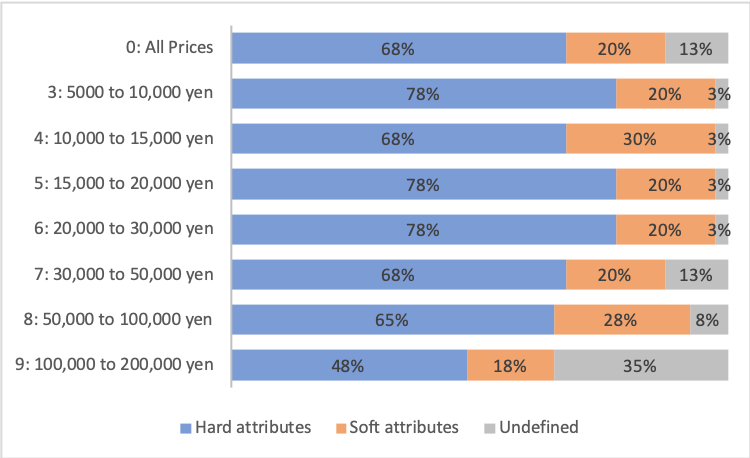
\includegraphics[width=\textwidth]{hard_soft_attr_zh_pos.png}
            \caption{Positive keywords}
        \end{subfigure}
        \begin{subfigure}[b]{0.45\textwidth}
            \includegraphics[width=\textwidth]{hard_soft_attr_zh_neg.png}
            \caption{Negative keywords}
        \end{subfigure}
    \caption{Percentages of hard and soft attributes of the top Chinese keywords for all price ranges}
    \label{fig:zh_hard_soft}
    \end{figure}


% \subsection{Chinese tourists - A big and clean space}\label{disc:zh}

% We found that mainland Chinese tourists are satisfied mostly by a big and clean space provided by the Japanese hotels. From inspecting random samples, we also find that this is mostly relating to the rooms. There are also many references to the public bathing facilities in the hotel. In Japan, there is what is called \textit{sent\=o}, which are artificially made public bathing facilities, on occasions including saunas and baths with unique qualities. On the other hand, there are natural hot springs, called \textit{onsen}. They can either be bathing in the natural source of the water or using the hot springs in artificially made bath facilities. It is a Japanese custom and culture that all customers use the facilities after cleaning themselves in a shower and go into the baths without any clothes. It can be a cultural shock for many tourists, but this is a fundamental attraction for many.

% From these two first ranking keywords (``big" and ``clean"), we can assert that room quality is the most critical satisfaction factor for Chinese customers. However, the word ``big" is widespread in the language and could be used in different contexts to point out positive and negative aspects. Since we are interested in how the word is a keyword of positive sentences, we took a small sample of the positively classified sentences that contained the word ``big" in Chinese. A team of Chinese speaking lab members then pointed out the usage of the word. Generally speaking, it was used for the spaciousness of rooms, bathtubs, and communal bath facilities. 

% One key component we found in Chinese customer satisfaction factors is the inclusion of breakfast within the hotel. While other food-related words were extracted, most of them were general, like “food” or “eating,” and in a lower ranking. In contrast, the word “breakfast” refers possibly to its inclusion in the hotel commodities, was frequently used in positive texts compared to other food-related words. A recommended strategy for hotel management is to invest in the inclusion or betterment of hotel breakfast. 

% \subsection{Western tourists - A friendly face, and absolutely clean}\label{disc:en}

% From the satisfaction factors of English-speaking tourists, we can see that at least three words relate to staff friendliness and services. The word ``staff" is the most frequently used word for satisfied customers, while ``helpful" and ``friendly" follow it lower in the list at the fourth and fifth place. Japanese high standards in hospitality very likely influenced this result.

% Aside from cleanliness, we can also observe the word ``working" is written higher on the list, as well as the word ``paper." We observed the samples, and it is often used with the expression ``paper-thin walls", which could mean the customers can easily hear their neighbors. Regarding the word ``working,'' we also took a sample of the texts to see its context. It seems to be related mostly to construction work near or at the facilities. Some cities in Japan (e.g., Osaka) are currently undergoing a large number of renovations, which are also extending to the hotel facilities. Customers staying in places in renovation or near a construction site can be expected to wake up to construction noises, have their view obstructed by metal bars, and other unpleasant experiences. Another keyword there is ``slow", which upon inspection of example reviews, we concluded that it reflects the speed of the Internet connection in the hotel rooms.

% An interesting detail of the keyword ranking is that the word ``comfortable" is high on the list of satisfaction factors and ``uncomfortable" high on the dissatisfaction factors. It seems that in general, western tourists are highly sensitive to comfort levels in the hotels and whether it reaches their expectations.


% \subsection{Tobacco, what's that smell?}\label{disc:tobacco}

% A concern for Western tourists was the smell of tobacco in their room. Upon manual inspection of a sample of reviews with this keyword, we found that the room was often advertised as non-smoking, yet, the smell permeated the room and curtains. Another common complaint was that there were no non-smoking facilities available at all. The smell of smoke can completely ruin some customers' stay and give a bad impression to review writers, which can lower the number of future customers. 

% However, in comparison, Chinese customers seem not to be bothered by this at all. We consulted studies involving the use of tobacco in different countries. Previous research states that 49 - 60\% of Chinese men (and 2.0 - 2.8\% of women) currently smoke or have smoked before, taken from a sample of \num[group-separator={,}]{170000} Chinese adults in 2013-2014, which is high compared to many English-speaking countries \cite[][]{zhang2019tobacco, who2015tobacco}.

% Japan itself has a polarized view on smoking, and despite being one of the world's largest tobacco markets, its use has been decreasing in recent years. Smoking in public spaces is prohibited in some wards of Tokyo (namely Chiyoda, Shinjuku, and Shibuya). However, it is generally only urged and not mandatory to have smoking restrictions in restaurants, bars, hotels, and public areas. However, there are many places where ``smoking rooms" are available to keep the smoke to an enclosed area and avoid bothering others. Despite this, businesses, especially those who cater to certain kinds of customers, will generally be discouraged from having smoking restrictions if they want to keep their clientele. If Japanese hotels want to cater to all kinds of customers, Western and Asian alike, they must provide spaces without tobacco smell. After all, even if it does not bother a few customers, the lack of smell would make it an appropriate space for all kinds of customers. 


% \subsection{Location, location, location}\label{disc:location}

% The location of the hotel, closeness to the subway and public transport, and availability of nearby shops were observed to be of importance to both Chinese and English-speaking tourists. While it was not the priority for either of them, we can assert that the hotel's location is a secondary but still important point in the hotel's satisfaction. However, since this is an external factor to the management of the hotel, it is not often considered in the literature. Upon inspection of examples from the data, we found that most customers were satisfied if the hotel was near to at least two other subjects: subway, train, and convenience stores. 

% Japan is a country with a peculiar public transport system. The rush hour makes for a subway filled to the brim with people in suits making their commute, and trains and subway stations in Tokyo create a confusing public transport map for a visitor. Buses are also available, although less used than the rail systems in the big cities. These three are unusually affordable in price. Then there are the more expensive transports, such as the bullet train \textit{shinkansen} for traveling across the country, and taxis. Taxis in Japan are a luxury compared to other countries. Where in less developed countries the taxi is the cheap method of transport of choice, in Japan, taxis are made to provide a high-quality experience, with a matching price. This means that for tourists, subway availability and maps or GPS applications, as well as a plan to travel the city, are of utmost necessity.

% Japanese convenience stores, on the other hand, are also famous worldwide. Japanese convenience stores are a haven for the traveler in need. It offers anything, from drinks and snacks to full meals, copy and scanning machines, alcohol, cleaning supplies, personal hygiene items, underwear, towels, international ATMs, and so on. If some trouble occurred, or a traveler forgot to pack a particular item, it is almost sure that they can find it.

% Therefore, considering that both transport systems and nearby shops are points of interest for Chinese and Western tourists, Japanese hotels have to carefully choose their location from the moment they are constructed. While not a top priority, this is a universal factor for both customer groups, and it can be an instant way to generate positive reviews.



% \section{Discussion}\label{discussion}

  % The results indicate that our hypothesis - Chinese and Western tourists have different priorities in hotel attributes that lead to their satisfaction and dissatisfaction - is correct. Furthermore, they indicate that, in the context of Japanese hospitality, only Western customers show satisfaction from staff and service amongst their top detected factors. Below we explore the possible interactions with \textit{Omotenashi}, what the differences between Chinese and Western tourists were, what is the possible cause for them, and what they imply for the industry. We also discuss the differences between managerial and environmental elements of the hotel and how they contribute to the satisfaction of customers in light of the results from our third hypothesis - Satisfaction and dissatisfaction stem from both internal (managerial) and external (environmental) attributes of the hotel.

  % \subsection{Western and Chinese tourists in the \textit{Omotenashi} environment}\label{disc:omotenashi}

    % To this day, scholars continue to correct our historical bias towards the west. In this time, studies have determined that different cultural backgrounds lead to different expectations, which in turn influence the satisfaction of tourists. Meaning, tourists of a particular culture will have different leading satisfaction factors across different destinations. However, Japan presents a particular environment. The spirit of hospitality and service, \textit{Omotenashi}, excels, and is considered the highest standard across the world. Can such an environment affect different cultures equally? Or is it only attractive to certain cultures? Our study brings light to these questions. 

    % Our results indicate that Western tourists are the most satisfied with friendly and helpful staff in Japan. As explained earlier in this paper, Japan is famous for its customer service all over the world. Respectful language and bowing are not exclusive to high priced hotels or businesses and can even be found in convenience stores. The level of hospitality in even the cheapest of convenience stores is starkly different from Westerner experiences. While it could be a culture shock to some, it is mostly seen positively. After all, the Japanese staff respectfully treats all customers. However, for some customers, this could be the best way they have been treated until that moment. We can also see that \cite{kozak2002} and \cite{shanka2004} have also found that hospitality and staff friendliness is a vital determinant in the satisfaction of Western tourists. 

    % However, we can see from the rest of the western keywords that a big part of the dissatisfaction with Japanese hotels stems from a lack of hygiene and room cleanliness. Although Chinese customers only had positive keywords about cleanliness, English-speaking customers have found many places unacceptable to their standards. The most common complaint regarding cleanliness was about the carpet, followed by complaints about cigarette stench, and general dirtiness. \cite{kozak2002} also found that hygiene and cleanliness were essential satisfaction determinants for Western tourists. However, in the previous literature, this was linked merely to satisfaction. In comparison, our research uncovered that words relating to cleanliness are mostly linked to dissatisfaction. Westerners could be said to have a high standard of room cleanliness when compared to their Chinese counterparts. 

    % According to previous research, we can see that Western tourists are already inclined to appreciate hospitality for their satisfaction. When presented with Japanese hospitality, this expectation is met and overcome. However, we can see from our results that Chinese tourists had less focus on hospitality, staff, or service and were more concerned with room quality. We could theorize that despite being presented with high standard hospitality, it is ignored. It could be that their culture does not hold the expectation initially. That is, when an expectation that is not held is met, the satisfaction that stems from this is less than if it was expected.

    % On the other hand, we have the phenomenon of a ``nice surprise'': When an unknown need is unexpectedly met, there is more satisfaction. It is necessary to note the difference between these two phenomenons. The ``nice surprise'' fulfills a need unexpectedly, while perhaps the hospitality grade in Japan is not fulfilling a high enough need for the Chinese population, resulting in less satisfaction. For greater satisfaction, the existence of a need being met is necessary. 

    % However, another possibility presents itself when we observe the Chinese tourists' dissatisfaction factors. Chinese tourists may have expectations about the treatment towards the Chinese visitors that are not being met, even in this high standard hospitality environment. Japan is known worldwide for their hospitality, but they are also known historically to be monolingual and have a relatively large language barrier \cite{heinrich2012making, coulmas2002japan}. While the Japanese effort to accommodate English speakers is slowly taking shape, Chinese accommodations can be lagging. Chinese language pamphlets, Chinese texts on instructions for the hotel room, and its appliances and features (e.g., T.V. channels, Wi-Fi setup), or just the treatment towards Chinese people could be examples. It is natural to be dissatisfied, since traveling in a strange land without knowing the language can be a daunting experience. \cite{ryan2001} also found that communication difficulty was one of the main reasons Chinese customers would state for not visiting again. It seems like this is a problem that is not singular to Japan.

    % Our initial question was whether the environment of high-grade hospitality would affect both cultures equally. This study brought us closer to the answer. On the one hand, there is a possibility that Chinese customers did have high-grade hospitality and did not get equally satisfied with Westerners. In that case, it appears that the difference stems from a psychological place. Expectation leads to satisfaction and a lack of expectation results in lesser satisfaction. On the other hand, there is also a possibility that Chinese customers are not receiving the highest grade of hospitality because of cultural friction between Japan and China. 

    % It is unclear from our results which of these could be the case. One thing is clear for hotel managers, however. Competing in \textit{Omotenashi} does include language services, especially in the international tourism industry. Better multilingual support can only improve that already high standard in Japan. Considering that most of the tourists in Japan come from other countries in Asia, this is an endeavor that truly can bring benefits to their investment. Proposals for this endeavor include hiring Chinese speaking staff, preparing pamphlets in Chinese, or have a translator application readily available with staff trained in interacting through an electronic translator.

  % \subsection{Managerial vs. Environmental satisfaction}\label{disc:man_env}

    % As we stated in section \ref{theory_satisfaction}, previous research is focused mostly on internal or managerial attributes of the hotel and their influence on customer satisfaction. Examples of managerial attributes include staff behavior, facilities, commodities, amenities, and appliances that can be improved within the hotel \cite[e.g.][]{shanka2004, choi2001}. However, external or environmental attributes, such as the location of the hotel relative to public transport and shops, language immersion of the country, noise pollution, or weather, are not usually analyzed in satisfaction studies. Because our study left the satisfaction factors to be decided statistically via customers' online reviews, we can see in their priorities the importance of those environmental or managerial attributes. 

    % From Table \ref{tab:hyp_man_env} and appendix Tables \ref{tab:man_env_pos} and \ref{tab:man_env_neg}, we can see that in regards to satisfaction, 40\% of keywords used by Chinese tourists are of an environmental nature (namely ``transportation", ``close", ``subway", and ``shopping"), while a lower 30\% is managerial in nature (and an undefined 30\%). However, two of these managerial words are all concentrated at the top of the list (``big", ``clean"). Chinese tourists could expect spaciousness and cleanliness when coming to Japan. That expectation could be caused by reputation, previous experiences, or cultural backgrounds. Some scholars argue that different cultures have different room size perceptions \cite{Saulton2017}. Although the study subjects are German and South Korean, the study presents the results as differences influenced by Asian and Western cultures. We argue that one country is not representative of others' cultures, so there can be differences between South Korea and China in room size perception. However, an interesting point appears. It could be that a different room size perception affects the satisfaction of Chinese tourists in contrast with Westerners. The dissatisfaction list for Western tourists could indicate that they perceive the rooms or bathtubs as small compared to Chinese tourists that praise them. We can compare these results with previous literature, where traveling Chinese tourists choose their destination based on several factors, including cleanliness, nature, architecture, and scenery \cite[][]{ryan2001}. These other few factors found in previous literature could be linked to the keyword ``environment" as well.

    % In comparison, English speakers are mostly satisfied with managerial attributes of the hotel, with keywords such as ``staff", ``clean," ``helpful," and ``friendly," to name a few. English-speaking customers also have managerial attributes at the very top of their list, except for the environmental nature of the location of the hotel. If one considers both Chinese and Western tourists' satisfaction, a hotel can improve in ways that will attract more customers in the future. If it was the other way around, and the satisfaction was related more with environmental attributes overall, hotels would have to compete solely on their location. 

    % For both customer groups, the main reason for dissatisfaction is pricing, which can be interpreted as a concern about value for money. A paper studying Chinese tourists found that they had this concern \cite[][]{truong2009}, but our results indicate that in the case of Japanese hotels, this is less of a cultural attribute, and has more to do with the pricing of hotels overall. The tourists coming to Japan could be both experienced travelers or first-time travelers, but the fact is that their expectation of the price for hotels was lower than what they found in Japan. In general, Japan is an expensive place to visit, which could impact this placement in the ranking. Space is scarce in Japan, and capsule hotels with cramped spaces of 2 x 1  meters cost around 3,000 to 6,000 yen per night. Bigger business hotel rooms are expensive, ranging from 5,000 to 12,000 yen per night. For comparison, hotels in the USA with a similar quality can be half the price. 

    % Similarly, most of the dissatisfaction is caused by issues that could be solved with improved management. Of course, this could be staff training (perhaps in language), hiring professional cleaning services for rooms with smoke smells, or improving the bedding, all of which can be costly. However, if hotels want to attract more customers, this paper provides a good guideline for which factors to consider first, and which ones will be best suited to which customer groups. 

    % Now, a point of interest in this study is the difference in how managerial and environmental factors concern Chinese and Western tourists. We can see that for Chinese customers, while the top positive keyword is managerial, the size of a room is hardly modifiable once the hotel's construction is complete. The second keyword follows as a managerial factor as well. Except, this time, hotel management can readily improve the cleanliness of their hotel. The rest of the positive keywords, however, are either undefined or environmental. Once the location and construction of the hotel are set, not much can be done to satisfy a Chinese tourist further. On the other hand, one can turn the dissatisfaction factors into satisfaction by focusing on those for improvement. As mentioned before, Chinese language availability is another managerial attribute that can be improved with investment in staff and training. 

    % Western tourists, on the other hand, are all around both satisfied and dissatisfied with mostly managerial factors, with a 50\% of the top 10 satisfaction factors and a 100\% of the top 10 dissatisfaction factors coming from managerial attributes. The room for improvement for Western tourists is more extensive than their Chinese counterparts, and as such, present a bigger investment opportunity. As mentioned earlier in this paper, Westerners are known as ``long-haul" customers, spending more than 45\% of their budget on hotel lodging. On the other hand, their Asian counterparts only spend 25\% of their budget on hotels \cite{choi2000}. With bigger returns on managerial improvements, it seems like investing in improving attributes that dissatisfy Western customers, such as cleanliness and removing tobacco smell. Making more hotel facilities tobacco-free and deodorizing the rooms can be a low-cost investment that could increase returns many times over. 

    % The opposite argument could also be made, however, that Chinese customers provide a more significant number of customers, even though they tend to spend less on lodging. Attracting a large number of Chinese customers can be a viable strategy for hotels. However, as mentioned before, they tend to focus more on environmental attributes, leaving language barrier-breaking as one of the few strategies to accomplish this.

    % The basic premise of this study is that different cultures lead to different expectations and satisfaction factors. This premise also plays a role in the differentiation between the preference of managerial or environmental attributes. Perhaps the cultural background of Chinese tourists emphasizes their surroundings and their place in nature and the environment. Chinese historical backgrounds of Confucianism, Taoism and Buddhism permeate the thought processes of Chinese populations. However, scholars argue that the changes in generations and their economic and recent history gives less importance to these concepts in their lives \cite{gao2017chinese}. However, one could argue that there is a Chinese cultural attribute that emphasizes the environment and the place one is in towards satisfaction, rather than the way one is treated. According to previous research, Chinese tourists are collectivist, while Westerners are individualists \cite{kim2000}. A more anthropocentric and individualistic Western culture could result in more of their expectations and priorities be related to how one is treated in social circumstances, rather than the environment one is in. 

  % \subsection{Implications for hotel managers}\label{disc:implications}

    % Our study presents two important conclusions: one about hospitality and cultural differences, and another about managerial decisions towards two different populations. Chinese tourists are not experiencing the best that \textit{Omotenashi} has to offer. Either they do not get much satisfaction from hospitality or feel that basic language and communication needs are not being met. On the other hand, Western tourists are elated with Japanese hospitality. The other conclusion is that managerial decisions will mostly benefit Western tourists, except that Chinese language improvements and breakfast inclusion can satisfy more Chinese customers. Japan is recently seeing an increase in Chinese students as well as Western students of universities. Hiring students as part-time workers could increase the language services of a hotel.

    % To satisfy both customer types, hotel managers need to invest in cleanliness, deodorizing, and making hotel rooms tobacco-free. It could also be recommended to invest in breakfast inclusion and multilingual services and staff preparedness to deal with Chinese and English speakers. Western tourists were also observed to have high standards in comfort, which can be improved upon managerially for better reviews. Perhaps it could be suggested to perform surveys of the bedding that is most comfortable for Western tourists. However, not all hotels can invest in all of these factors simultaneously. Our results suggest that satisfying cleanliness needs can satisfy both customer types and that a low-cost investment could be to make the facilities tobacco-free. 

    % Environmental factors, while not manageable after a hotel has finished its construction, are essential to consider for managers as well. As previously stated, transport systems and nearby shops are points of interest for both Chinese and Western tourists. Japanese hotel managers have to consider the location and surroundings since before the hotel is constructed. A suggestion could be to purchase land and start the construction after plans to make new subway lines are made. 

    % It is left to the managers to consider their business model for the next strategy. One option could be attracting more Chinese customers in number with their observed low budgeting. Another could be attracting more high budget Western customers is on par with their business model. For example, investing more on cleanliness could improve on Western customers looking for high-quality lodging, even though the price per night would increase.

% \section{Limitations and Future Work}\label{limitations}

  % This paper is not without its limitations. We analyzed keywords of satisfaction and dissatisfaction statistically based on whether they appeared on satisfied reviews or dissatisfied ones. Following that, we attempted to understand the context that these words were being used in by using a dependency parser and observing the related nouns. However, the study is limited in that it only analyzes the words directly related to each keyword, and doesn't follow the upstream or downstream path down further connections. This means that if the words are used in combination with other keywords we did not trace the effects of multiple contradicting statements. For example, in the sentence "The room is good but the food is lacking", we would extract "good food" and "lacking food", but do not consider the fact that both occurred in the same sentence.

  % In this study, we analyzed the differences in customers expectations at different levels of \textit{Omotenashi} by dividing our data into price ranges. However, in the same price range, say the high expenses ones, we can find both a western style five stars resort as well as a high end Japanese style \textit{Ryokan}. Services offered in these hotels are very high quality, although very different in nature. However, most of our database is focused on the middle range priced hotels, which is comparably less varied in service, although still there is a divide between western and Japanese style hotels.

  % Another limitation is that a large portion of the Asian tourists coming to Japan is Taiwanese and Korean. We could not analyze these populations because our team members do not know those languages. Aside from that, because of the nature of the data collected, further typology analysis could not be made (for example, Chinese men and women of different ages or their Westerner counterparts).

  % In future work, we plan to investigate further into this topic. We plan to extend our data to research for different trends for different regions of Japan and in different kinds of hotels, as well as between customers traveling alone or in groups, for fun or work. Another point of interest in the future of this study is to use word clusters with similar meanings instead of single words. 

% \section{Conclusion}\label{conclusion}

  % In this study, our objective was to analyze the differences in satisfaction and dissatisfaction between Chinese and English-speaking customers of Japanese hotels. We extracted keywords from their online reviews uploaded to the portal sites \textit{Ctrip} and \textit{TripAdvisor} using Shannon's entropy calculations. We used these keywords for sentiment classification via an SVC. 

  % In the context of Japanese hospitality, we found that Western tourists had the most satisfaction with staff behavior, confirming our hypothesis \ref{hyp:omotenashi_en}. However, we found that Chinese customers had other concerns than hospitality when studying their satisfaction. As such, our hypothesis \ref{hyp:omotenashi_zh} is rejected. Since both cultures have a different reaction to this environment of hospitality, our hypothesis \ref{hyp:omotenashi_both} is confirmed. From this, we discussed two possible theories on why Chinese tourists respond differently to Westerners in this environment of \textit{Omotenashi}. One theory is that they are not being treated well enough, and this environment is not compatible with them because of language or culture barriers. The second possible theory is that they react differently to hospitality since they do not have the same expectations to be satisfied in the same way. We theorize that a lack of expectations could result in lessened satisfaction, even if the same service is presented.

  % Lastly, we measured the amount of satisfaction and dissatisfaction factors that were referring to managerial attributes of a hotel or environmental attributes of the hotel. Managerial attributes are those that they can be changed via managerial decisions without relocating. On the other hand, environmental attributes are things like location, closeness to shops, or public transport. We found that both are included in the satisfaction and dissatisfaction of both customer groups, confirming our hypothesis \ref{hyp:man_env}. We also found that most of the Western customer satisfaction (50\% of the top 10 words) and dissatisfaction (100\% of the top 10 words) stems from managerial attributes of the hotel.

  % In contrast, environmental attributes only make for a smaller portion of the factors (40\% of the top 10 satisfaction keywords). In the case of Chinese customer satisfaction, the top of the list was managerial (30\% of the top 10 words), and a more significant portion, although lower in its ranking, was environmental (40\%). For Chinese customer dissatisfaction, however, 71.4\% of the keywords were managerial, while the other 28.6\% were environmental. We discussed how these distributions in managerial or environmental factors having priorities in either population could lead to different management strategies. One possible approach is to try to improve the satisfaction levels of Chinese tourists, who dedicate less percentage of their budget to hotels but are more abundant in number. They are less satisfied with managerial factors but have an identifiable method of improving satisfaction by lessening language barriers and providing breakfast. Another approach we discussed was focusing on the cleanliness and comfort that Western tourists expect, as well as making the hotels tobacco-free. With this strategy, we favor ``long-haul'' Western tourists who spend almost half of their budget on hotels. While Westerners are less in number than Chinese tourists, it could prove to have more substantial returns. The reason for this being that Chinese customers also favor cleanliness as a satisfaction factor, and both populations could be pleased. In this paper, we provide results and discussion that can be utilized as a guideline for managerial decisions when considering Chinese and Western tourists in Japan, and we can observe their stark differences and shared attributes. 

\begin{acknowledgements}

  During our research, we received the commentary and discussion by our dear colleagues necessary to understand particular cultural aspects that could influence the interpretation of the data. We would like to show gratitude to Mr. Liangyuan Zhou, Ms. Min Fan, and Ms. Eerdengqiqige for this.

  We would also like to show gratitude to Ms. Aleksandra Jajus, from whom we also received notes on the editing and commentary on the content of our manuscript.

  \medskip

  Funding: This work was supported by the Japan Construction Information Center Foundation (JACIC).

  \medskip

  Conflict of interest: none

\end{acknowledgements}

% \section*{References}

\bibliography{bibfile-emotion}

\end{document}
